% ---------------
% PREAMBLE
% ---------------
\newif\iflatextortf

\iflatextortf
	% tell latex2tortf if this is an article or report
 	\documentclass[12pt,letterpaper]{article}
	% File NRELLatex2rtf.tex

% set margins
\usepackage[margin=1 in,letterpaper]{geometry}

% use citations
\usepackage[sort]{natbib}

% change the heading of the bibliography
\renewcommand{\bibsection}{\section{References}}

% redefine \pdftooltip so that it behaves differently with and without latextortf
\newcommand{\pdftooltip}[3][]{#2}

%redefine the checkmark
\newcommand{\checkmark}{y\relax}

% redefine booktabs commands
\newcommand{\toprule}{\hline}
\newcommand{\midrule}{\hline}
\newcommand{\bottomrule}{\hline}

% redefine \href
\newcommand{\href}[2]{#1~ (\url{#2})}

% redefine \subfloat to match the \subfigure environment
\usepackage{subfigure}
\makeatletter
\newcommand{\subfloat}[2][]{\subfigure{\textit{Subcaption: \protect{#1}}}{#2}}
%\newcommand{\subfloat}[3][]{\subfigure{#1}{#2}{#3}}
% note that we can only have one '\label' in a figure environment
\makeatother

\newcommand{\subref}[1][]{\ref{#1}}

% redefine \todo so that it gives something useful
\newcommand{\todo}[2][]{\textbf{To Do:}~#2}

% deal with index entries:
\newcommand{\index}[1]{}
\else
	%\documentclass[report,tagged]{nrel}
	\documentclass[report]{nrel}
\fi


\def\directory{Figure/}
\usepackage{pdfpages}
\usepackage{listings}

% -----------------------------------
% DOCUMENT PROPERTIES
% -----------------------------------
\title{BeamDyn User's Guide}
\author{Q. Wang, J. Jonkman, M. Sprague, and B. Jonkman}

% -------------------------------------
% DOCUMENT STARTS HERE
% -------------------------------------
\begin{document}

\frontmatter
%\chapter*{Executive Summary}
This document is a guide to writing documents for publication by NREL using the LaTeX document preparation system. LaTeX is not WYSIWYG and has different reviewing and editing tools compared to typical word processing software. For this reason special care has to be taken when preparing NREL documents in LaTeX. This document serves both as a guide to implementing NREL's style and formatting guidelines in LaTeX, and as a template. This document is intended for people with some familiarity with LaTeX.
\chapter*{Preface}
This document offers a quick reference guide for the BeamDyn software program. It is intended to be used by the general user in combination with other FAST manuals. The manual will be updated as new releases are issued and as needed to provide further information on advancements or modifications to the software.
\chapter*{Acknowledgments}
The authors are grateful to the U.S. Department of Energy Wind and Water Power Program  and the NREL Laboratory Directed Research and Development (LDRD) program through the grant ``High-Fidelity Computational Modeling of Wind-Turbine Structural Dynamics''
for supporting the development of this software.


\mainmatter
\tableofcontents
\listoffigures
\listoftables
\lstset{language=Fortran} 

\chapter{Introduction}
BeamDyn is a time-domain structural-dynamics module for slender structures created by the National Renewable Energy Laboratory (NREL) through U.S.\ Department of Energy Wind and Water Power Program support. 
The module has been coupled into the FAST aero-hydro-servo-elastic wind turbine multi-physics engineering tool where it used to model blade structural dynamics. 
%BeamDyn is designed to analyze beams that are made of composite materials, allowing for initial curvature and twist, and subject to large displacement and rotation deformations. BeamDyn can also be used for static analysis of beams.
The BeamDyn module follows the requirements of the FAST modularization framework (ADD REF), couples to FAST version 8, and provides new capabilities for modeling initially curved and twisted composite wind turbine blades undergoing large deformation. 
BeamDyn can also be driven as a stand-alone code to compute the static and dynamic responses of slender structures (blades or otherwise) under prescribed boundary conditions uncoupled from FAST.

The model underlying BeamDyn is the geometrically exact beam theory (GEBT) \mas{ADD REF}.   
GEBT supports full geometric nonlinearity and large deflection, with bending, torsion, shear, and extensional degree-of-freedom (DOFs); anisotropic composite material couplings (using full $6 \times 6$ mass and stiffness matrices, including bend-twist coupling); and a reference axis that permits blades that are not straight (supporting built-in curve, sweep, and sectional offsets). 
The GEBT beam equations are discretized in space with Legendre spectral finite elements (LSFEs).  
LFSEs are {\it p}-type elements that combine the accuracy of global spectral methods with the geometric modeling flexibility of the {\it h}-type finite elements (FEs). 
For smooth solutions, LSFEs have exponential convergence rates compared to low-order elements that have algebraic convergence. 
Two spatial numerical integration schemes are implemented for the finite element inner products: reduced Gauss quadrature and trapezoidal-rule integration.  
Trapezoidal-rule integration is appropriate when a large number of sectional properties are specified along the beam axis, for example, in a long wind turbine blade with material properties that vary dramatically over the length.  
Time integration of the BeamDyn equations of motion is achieved through the implicit generalized-$\alpha$ solver, with user-specified numerical damping.
The combined GEBT-LSFE  approach permits users to model a long, flexible, composite wind turbine blade with a single high-order element.  
Given the theoretical foundation, powerful numerical tools introduced above, BeamDyn can solve the complicate nonlinear composite beam problem in an efficient manner. For example, it was recently shown that a grid-independent dynamic solution of a 50 m composite wind turbine blade and with dozens of cross-section stations could be achieved with a 
single $6^{th}$-order LSFE \mas{Add Reference; SciTech Paper}

When coupled with FAST, loads and responses are transferred between BeamDyn, ElastoDyn, ServoDyn, and AeroDyn via the FAST driver program (glue code) to enable aero-elasto-servo interaction at each coupling time step. 
There is a separate instance of BeamDyn for each blade. 
At the root node, BeamDyn inputs are six displacements (three translations and three rotations), six velocities, and six accelerations; the root node outputs are six reaction forces (three translational forces and three moments). 
BeamDyn also outputs the blade displacements, velocities, and accelerations along the beam length, which are used by AeroDyn to calculate the local aerodynamic loads that are used as inputs for BeamDyn. 
In addition, BeamDyn can calculate member internal reaction loads, as requested by the user. 
Please refers to Figure~\ref{fig:FlowChart} for the coupled interactions between BeamDyn and other modules in FAST. 
When uncoupled from FAST, the root motion and applied loads are specified via a stand-alone BeamDyn driver code.
\begin{figure}
    \centering
    \includegraphics[width = \textwidth,angle = 0]{\directory FlowChart.jpg}
    \caption{Coupled interaction between BeamDyn and FAST}
    \label{fig:FlowChart}
\end{figure}

The BeamDyn input file defines the blade geometry, cross-sectional material mass, stiffness, and damping properties, FE resolution, and other simulation- and output-control parameters. 
The blade geometry is defined through a curvilinear blade reference axis by a series of key points in three-dimensional (3D) space along with the initial twist angles at these points. 
Each \textit{member} contains at least three key points for the cubic spline fit implemented in BeamDyn; each member is discretized with a single LSFE with a parameter defining the order of the element. 
Note that the number of key points defining the member and the order ($N$) of the LSFE are independent.
LSFE nodes, which are located at the $N+1$ Gauss-Legendre-Lobatto points, are not evenly spaced along the element; node locations are generated by the module based on the mesh information. 
Blade properties are specified in a non-dimensional coordinate ranging from 0.0 to 1.0 along beam axis and are linearly interpolated between two stations if needed by the spatial integration method. 
The BeamDyn applied loads can be either distributed loads specified at quadrature points,  concentrated loads specified at FE nodes, or a combination of the two.  

This document is organized as follows. Section~\ref{sec:Run} details how to obtain the BeamDyn and FAST software archives and run either the stand-alone version of BeamDyn or BeamDyn coupled to FAST. Section~\ref{sec:InputFiles} describes the BeamDyn input files. Section~\ref{sec:OutputFiles} discusses the output files generated by BeamDyn. Example input files are shown in Appendix~\ref{sec:AppDriver}, \ref{sec:AppPrimary}, and  \ref{sec:AppBlade}. A summary of available output channels is found in Appendix~\ref{sec:AppOutputChannel}

\chapter{Running BeamDyn}
\label{sec:Run}
This section discusses how to obtain and execute BeamDyn from a personal computer. Both the stand-alone version and the FAST-coupled version of the software are considered.

\section{Downloading the BeamDyn Software}
There are two forms of the BeamDyn software to choose from: stand-alone and coupled to the FAST simulator. Alghough the user may not necessarily need both forms, he/she would likely need to be familiar with and run the stand-alone model if building a model of the blade from scratch. The stand-alone version is also helpful for model troubleshooting and may benefit users who are interested in conducting aero-hydro-servo-elastic simulations of onshore/offshore wind turbines. For this reason, BeamDyn can be obtained from two different repositories: one for the stand-alone BeamDyn and one for the coupled solution through FAST.

\subsection{Stand-Alone BeamDyn Archive}
Users can download the stand-alone BeamDyn archive from our Web server at \url{https://nwtc.nrel.gov/BeamDyn}. The file has a name similar to {\it BD\_v1.00.00a.exe}, but may have a different version number. The user can then download the self-extracting archive ({\it .exe}) to expand the archive into a folder he/she specifies.

\begin{figure}
    \centering
     \includegraphics[width = 4.0 in]{\directory BeamDyn_archive.eps}
     \caption{WinZip self-extractor main window}
     \label{fig:BDSelfExtractor}
\end{figure}

The archive contains the \textbf{\textit{bin}}, \textbf{\textit{CertTest}}, \textbf{\textit{Compiling}}, \textbf{\textit{Documentation}}, and \textbf{\textit{Source}} folders. The \textbf{\textit{bin}} folder includes the main executable file, \textit{BeamDyn\_win32.exe}, which is used to execute the stand-alone BeamDyn program. The \textbf{\textit{CertTest}} folder contains a collection of sample BeamDyn input files and driver input files that can be used as templates for the user's own models. This manila may be found in the \textbf{\textit{Documentation}} folder. The \textbf{\textit{Compling}} folder contains files for compiling the stand-alone \textit{BeamDyn\_v1.00.00.exe} file with either Visual Studio or gFortran. The Fortran source code is located in the \textbf{\textit{Source}} folder.

\subsection{FAST Archive}
Download the FAST archive, which includes a coupling to BeamDyn, from our Web server at \url{https://nwtc.nrel.gov/FAST8}. The file has a name similar to \textit{FAST\_v8.12.00.exe}, but may have a different version number. Run the downloaded self-extracting archive ({\it .exe}) to expand the archive into a user-specified folder. The FAST executable file is located in the archive's \textbf{{\it bin}} folder. Example models using the NREL 5-MW reference turbine are located in the \textbf{{\it CertTest}} folder.

\section{Running BeamDyn}
\subsection{Running the Stand-Alone BeamDyn Program}
The stand-alone BeamDyn program, {\it BeamDyn\_v1.00.00.exe}, simulates static and dynamic responses of the user's input model, without coupling to FAST. Unlike the coupled version, the stand-alone software requires the use of a driver file in addition to the primary  and blade BeamDyn input files. This driver file specifies inputs normally provided to BeamDyn by FAST, including motions of the blade root and externally applied loads. Both the BeamDyn summary file and the results output file are available when using the stand-alone BeamDyn (see Section~\ref{sec:OutputFiles} for more information regarding the BeamDyn output files).

Run the stand-alone BeamDyn software from a DOS command prompt by typing, for example:
\begin{verbatim}
>BeamDyn_v1.00.00.exe Dvr_5MW_Dynamic.inp
\end{verbatim}
where, {\it Dvr\_5MW\_Dynamic.inp} is the name of the BeamDyn driver input file, as described in Section~\ref{sec:DriverInputFile}.

\subsection{Running BeamDyn Coupled to FAST}
Run the coupled FAST software from a DOS command prompt by typing, for example:
\begin{verbatim}
>FAST_v.8.12.00.exe Test26.fst
\end{verbatim}
where {\it Test26.fst} is the name of the primary FAST input file. This input file has a feature switch to enable or disable the BeamDyn capabilities within FAST, and a corresponding reference to the BeamDyn input file. See the documentation supplied with FAST for further information.





\chapter{Input Files}
\label{sec:InputFiles}
Users specify the blade model parameters; including its geometry, properties, and FE and output control parameters; via a primary BeamDyn input file and a blade property input file. When used in stand-alone mode, an additional driver input file is required. This driver file specifies inputs normally provided to BeamDyn by FAST, including simulation range, root motions (initial conditions), and externally applied loads.

No lines should be added or removed from the input files, except in tables where the number of rows is specified.

\section{Units}
BeamDyn uses the SI system (kg, m, s, N). Angles are assumed to be in radians unless otherwise specified.

\section{BeamDyn Driver Input File}
\label{sec:DriverInputFile}
The driver input file is only needed for the stand-alone version of BeamDyn and contains inputs that are normally set by FAST, and that are necessary to control the simulation for uncoupled models. 

The driver input file begins with two lines of header information, which is for the user but is not used by the software. If BeamDyn run in the stand-alone mode, the results output file will be prefixed with the same name of this driver input file.

A sample BeamDyn driver input file is given in Appendix \ref{sec:AppDriver}

\subsection{Simulation Control Parameters}
\textbf{\textit{t\_initial} } and \textbf{\textit{t\_final} } specify the starting time of the simulation and ending time of the simulation, respectively. \textbf{\textit{dt} } specifies the time step size.

\subsection{Gravity Parameters}
\textbf{\textit{Gx} }, \textbf{\textit{Gy} }, and \textbf{\textit{Gz} } specify the components of gravity vector along $X$, $Y$, and $Z$ directions in the global coordinate system, respectively.  In FAST, this is normally 0, 0, and -9.80665.

\subsection{Inertial Frame Parameters}
This section defines the relation between two inertial frames, the global coordinate system and initial blade reference coordinate system. \textbf{\textit{GlbPos(1)} }, \textbf{\textit{GlbPos(2)} }, \textbf{\textit{GlbPos(3)} } specifies three components of the initial global position vector along $X$, $Y$, and $Z$ directions resolved in the global coordinate system, see Figure \ref{fig:Frame}. And the following $3 \times 3$ direction cosine matrix (DCM) relates the rotations from global coordinate system to blade coordinate system. 

\begin{figure}
    \centering
    \includegraphics[width = 4.0 in]{\directory Frame.eps}
    \caption{Global and blade coordinate systems in BeamDyn}
    \label{fig:Frame}
\end{figure}

\subsection{Floating Blade Reference Frame Parameters}

This section specifies the parameters that defines the floating blade reference frame, which is a body-attached floating frame and the blade root is cantilevered at the origin of this frame. The floating blade reference fame is assumed to be in a constant rigid-body rotation mode about the origin of the global coordinate system, that is,
\begin{equation}
   \label{RootVelocity}
   v_r = \omega_r \times r_t
\end{equation}
where $v_r$ is the root (origin of the floating blade reference frame) translational velocity vector; $\omega_r$ is the constant root (origin of the floating blade reference frame) angular velocity vector; and $r_t$ is the global position vector introduced in the previous section at instant $t$, see Figure~\ref{fig:Frame}. It is pointed out that the floating blade reference frame coincides with the initial floating blade reference frame at the beginning $t=0$. \textbf{\textit{RootVel(4)} }, \textbf{\textit{RootVel(5)} }, and \textbf{\textit{RootVel(6)} } specify the three components of the root angular velocity vector about  $X$, $Y$, and $Z$ axises in global coordinate system, respectively.  \textbf{\textit{RootVel(1)} }, \textbf{\textit{RootVel(2)} }, and \textbf{\textit{RootVel(3)} }, which are the three components of the root translational velocity vector along  $X$, $Y$, and $Z$ directions in global coordinate system, respectively, are calculated based on Eq.~\ref{RootVelocity}. BeamDyn can handle more complicate root motions by change the part, for example, in $BD\_InputSolve$ subroutine in the Drvier\_Beam.f90:
\begin{lstlisting}[frame=single]
   u%RootMotion%RotationVel(:,:) = 0.0D0
   u%RootMotion%RotationVel(1,1) = IniVelo(5)
   u%RootMotion%RotationVel(2,1) = IniVelo(6)
   u%RootMotion%RotationVel(3,1) = IniVelo(4)
   u%RootMotion%TranslationVel(:,:) = 0.0D0
   u%RootMotion%TranslationVel(:,1) = &
   MATMUL(BD_Tilde(real(u%RootMotion%RotationVel(:,1),BDKi)),temp_rr)
\end{lstlisting}
where $IniVelo(5)$, $IniVelo(6)$, and $IniVelo(4)$ are the three components of the root angular velocity vector about  $X$, $Y$, and $Z$ axises in global coordinate system, respectively; $temp$\_$rr$ is the global position vector at instant $t$.

The blade is initialized in the rigid-body motion mode, i.e., based on the root velocity information defined in this section and the position information defined in the previous section, the motion of other points along the blade are initialized as
\begin{align}
    \label{IniRootAcc}
    a_{r0} &= \omega_r \times (\omega_r \times r_0) \\
    \label{IniTraVel}
    v_0 &= v_{r0} + \omega \times P \\
    \label{IniAngVel}
    \omega_0 &= \omega_r
\end{align}
where $a_{r0}$ is the initial root translational acceleration vector; $v_0$ and $\omega_0$ the initial translational and angular velocity vectors along blade other than the root, respectively; and $P$ is the position vector along the blade relative to the root. 

\subsection{Applied Load}
This section defines the applied loads, including distributed and tip concentrated loads, for the analysis. The first six entries \textbf{\textit{DistrLoad(i)} }, $i \in [1,6]$, specify three components of uniformly distributed force vector and three components of uniformly distributed moment vector in the global coordinate systems, respectively. The following six entries \textbf{\textit{TipLoad(i)} }, $i \in [1,6]$, specify three components of concentrated tip force vector and three components of concentrated tip moment vector in global coordinate system, respectively. The distributed load defined in this section is assumed to be uniform along the blade and constant throughout the simulation; the tip load is a constant concentrated load applied at the tip of a blade. 

BeamDyn is capable of handling more complex loading cases, for example, the time-dependent loads, through customizing of the source code (requiring a recompile of stand-alone BeamDyn). The user can define such loads in the \textit{BD\_InputSolve} solve in the Driver\_Beam.f90 file, which is called every time step. The following section can be modified to define the concentrated load at each FE node:

\begin{lstlisting}[frame = single]
   ! Define concentrated force vector
   u%PointLoad%Force(:,:)  = 0.0D0
   ! Define concentrated moment vector
   u%PointLoad%Moment(:,:) = 0.0D0
\end{lstlisting}
where the first index in each array ranges from 1 to 3 for load vector components along three directions and the second index of each array ranges from 1 to  \textbf{\textit{node\_total} }, where the latter is the total number of FE nodes. For example, a sinusoidal force along the $X$ direction applied at the $2^{nd}$ FE node can be defined as
\begin{lstlisting}[frame = single]
   ! Define concentrated force vector
   u%PointLoad%Force(:,:) = 0.0D0
   u%PointLoad%Force(1,2)  = 1.0D+03*SIN((2.0*pi)*t/6.0 )
   ! Define concentrated moment vector
   u%PointLoad%Moment(:,:) = 0.0D0
\end{lstlisting}
with $1.0D+03$ the amplitude and $6.0$ the period.

Similar to the concentrated load, the distributed loads can be defined in the same subroutine

\begin{lstlisting}[frame = single]
   IF(p%quadrature .EQ. 1) THEN
       DO i=1,p%ngp*p%elem_total+2
           u%DistrLoad%Force(1:3,i) = InitInput%DistrLoad(1:3)
           u%DistrLoad%Moment(1:3,i)= InitInput%DistrLoad(4:6)
       ENDDO
   ELSEIF(p%quadrature .EQ. 2) THEN
       DO i=1,p%ngp
           u%DistrLoad%Force(1:3,i) = InitInput%DistrLoad(1:3)
           u%DistrLoad%Moment(1:3,i)= InitInput%DistrLoad(4:6)
       ENDDO
   ENDIF
\end{lstlisting}
where p\%ngp is the number of quadrature points; InitInput\%DistrLoad(:) is the constant uniformly distributed loads BeamDyn reads from the driver input file, and p\%elem\_total is the total number of elements. The user can modify ``InitInput\%DistrLoad(:)" to define the loads based on need. 

It is pointed out that the distributed loads are defined at the quadrature points for numerical integrations. For example, if Gauss quadrature is chosen (p\%quadratrure .EQ. 1), then the distributed loads are defined at Gauss points plus the two end points of the beam (root and tip). 

\subsection{Primary Input File}
 \textbf{\textit{InputFile} } is the file name of the primary BeamDyn input file. This name should be in quotations and can contain an absolute path or a relative path. 
 
 

\section{BeamDyn Primary Input File}

The BeamDyn primary input file defines the blade geometry, FE and simulation options, output channels, and name of the blade input file. The geometry of the blade is defined by key point coordinates and initial twist angles (in units of degree) in the local blade coordinate system (IEC standard blade system where Z$_r$ is along blade axis from root to tip, X$_r$ directs normally toward the suction side, and Y$_r$ directs normally toward the trailing edge).

The file is organized into several functional sections. Each section corresponds to an aspect of the BeamDyn model.

A sample BeamDyn primary input file is given in Appendix \ref{sec:AppPrimary}

The primary input file begins with two lines of header information, which is for the user but is not used by the software.

\subsection{Simulation Controls}

User can set the \textbf{\textit{Echo} } flag to ``TURE" to have BeamDyn echo the contents of the BeamDyn input file (useful for debugging errors in the input file). 

\textbf{\textit{Analysis\_Type}} specifies the type of an analysis. In the current version, there are two options: 1) static analysis, and 2) dynamic analysis. If BeamDyn is run in coupled FAST mode, this entry can be only set to 2, i.e., for dynamic analysis.

\textbf{\textit{rhoinf}} specifies the numerical damping parameter (spectral radius of the amplification matrix) in the range of $[0.0,1.0]$ used in the generalized-$\alpha$ time integrator implemented in BeamDyn for dynamic analysis. For $\textbf{\textit{rhoinf}}  = 1.0$, no numerical damping is introduced and the generalized-$\alpha$ scheme is identical to the Newmark scheme; for $\textbf{\textit{rhoinf}}  = 0.0$, maximum numerical damping is introduced to help with convergence.

\textbf{\textit{Quadrature}} specifies the spatial numerical integration scheme. There are two options: 1) Gauss quadrature; and 2) Trapezoidal quadrature. It is pointed out that in the current version, the Gauss quadrature is implemented in reduced form to improve efficiency and avoid shear locking. In the trapezoidal quadrature, only one member (FE element) can be defined in the following GEOMETRY section of the primary input file.

\textbf{\textit{Refine}} specifies a refinement parameter used in trapezoidal quadrature. A value greater than unity will split the space between two input stations into Refine number of segments.The keyword ``DEFAULT'' may be used to set it to 1, i.e., no refinement is needed. This entry is not used in Gauss quadrature.   

\textbf{\textit{N\_Fact}} specifies a parameter used in the modified Newton-Ralphson scheme. If $\textbf{\textit{N\_Fact}} = 1$ a full Newton iteration scheme is used, i.e., the global stiffness matrix is computed and factorized at each iteration; if $\textbf{\textit{N\_Fact}} >  1$ a modified Newton iteration scheme is used, i.e., the global stiffness matrix is computed and factorized every \textbf{\textit{N\_Fact}} iterations  within each time step. The keyword ``DEFAULT'' set $\textbf{\textit{N\_Fact}} = 5$.

\textbf{\textit{DTBeam}} specifies the fixed time step of the time-integration in seconds. The keyword ``DEFAULT'' may be used to indicate that the module should employ the time step prescribed by the driver code (FAST/stand-alone driver program).

\textbf{\textit{NRMax}} specifies the maximum number of iterations in the Newton-Ralphson scheme. If convergence is not reached within this number of iterations, BeamDyn returns an error message and terminates the simulation. The keyword ``DEFAULT'' sets $\textbf{\textit{NRMax}} = 10$.

\textbf{\textit{Stop\_Tol}} specifies a tolerance parameter used in convergence criteria of a nonlinear solution that is used for the termination of the iteration. The keyword ``DEFAULT'' sets $\textbf{\textit{Stop\_Tol}} = 1.0E-05$.

\subsection{Geometry Parameter}

The blade beam model is composed of several {\it members} in series and each member is defined by at least three key points in BeamDyn. A cubic-spline-fit pre-processor implemented in BeamDyn automatically generates the member based on the key points and then interconnects the members into a blade. There is always a shared key points at adjacent members; therefore the total number of key points is related to number of members and key points in each member.

\textbf{\textit{Member\_Total}} specifies the number of beam members used in the structure.

\textbf{\textit{KP\_Total}} specifies the total number of key points used to define the beam members. 

The following section contains \textbf{\textit{Member\_Total}} lines. Each line has two integers providing the member number (must be 1, 2, 3, etc., sequentially) and the number of key points in this member, respectively. It is noted that the number of key points in each member is not independent of the total number of key points and they should satisfy the following equality:
\begin{equation}
    \label{Keypoint}
    KP_{t} = \sum_{i=1}^{M_t} n_i - M_t +1
\end{equation}
where $KP_{t}$ is the total number of key points, $M_t$ is the total number of members, and $n_i$ is the number of key points in the $i^{th}$ member. Because cubic splines are implemented in BeamDyn, $n_i$ must be greater than or equal to three. Figure \ref{fig:Geometry1} shows two cases for member and key point definition.
\begin{figure}[htp]
\centering
    \subfigure[Case 1 \label{Geometry1:Case1}]{\includegraphics[width=4.0in]{\directory Geometry_Member1.eps}}\\
    \subfigure[Case 2 \label{Geometry1:Case2}]{\includegraphics[width=4.0in]{\directory Geometry_Member2.eps}}
    \caption{Member and key point definition. Case 1: one member defined by four key points; and Case 2: two members defined by six key points.}
    \label{fig:Geometry1}
\end{figure}

The next section defines the key points information. Each key point is defined by three physical coordinates in IEC standard blade coordinate system along with a structural twist angle in the unit of degrees. The structural twist angle is also following the IEC standard which is defined as the twist about the negative Z axis. The key points are entered sequentially and there should be a total of \textbf{\textit{KP\_Total}}  lines for BeamDyn to read in the information, after two header lines.

\subsection{Mesh Parameter}

\textbf{\textit{Order\_Elem}} specifies the order of shape functions for each finite element. Because LSFEs are adopted in BeamDyn, it is recommended to refine the mesh by increasing the order of elements ($p$-type) instead of increasing the number of elements. For Gauss quadrature, \textbf{\textit{Order\_Elem}} should be greater than one. 

\subsection{Material Parameter}

\textbf{\textit{BldFile}} is the file name of the blade input file. This name should be in quotations and can contain an absolute path or a relative path.

\subsection{Pitch Actuator Parameter}

In this release, the pitch actuator implemented in BeamDyn is not available. The \textbf{\textit{UsePitchAct}} should be set to "FALSE" in this version, whereby the input blade-pitch angle prescribed by the driver code is used to orient the blade directly. \textbf{\textit{PitchJ}}, \textbf{\textit{PitchK}}, and \textbf{\textit{PitchC}} specify the pitch actuator inertial, stiffness, and damping coefficient, respectively. In future releases, specifying \textbf{\textit{UsePitchAct}} $=$ TRUE will enable a second-order pitch actuator, whereby the pitch angular orientation, velocity, and acceleration are determined by the actuator based on the input blade-pitch angle prescribed by the driver code.

\subsection{Outputs}

In this section of the primary input file, the user sets flags and switches for the desired output behavior.

Specifying \textbf{\textit{SumPrint}} $=$ TRUE causes BeamDyn to generate a summary file with name \textit{\textbf{PrimaryInputFile}.sum}. See Section~\ref{sec:SumFile} for summary file details.

\textbf{\textit{OutFmt}} parameter controls the formatting of the results within the stand-alone BeamDyn's output file. It needs to be a valid Fortran format string, but  BeamDyn currently does not check the validity. This input is unused when BeamDyn is used coupled to FAST.

\textbf{\textit{NNodeOuts}} specifies the number of nodes to output to file. Currently, BeamDyn can output quantities at a maximum of nine nodes. 

\textbf{\textit{OutNd}} is a list \textbf{\textit{NNodeOuts}} long of node numbers between 1 and $node_total$ (total number of FE nodes), separated by any combination of commas, semicolons, spaces, and/or tabs.   The nodal positions are given in the summary file, if output.

The \textbf{\textit{OutList}} block contains a list of  output parameters. Enter one or more lines containing quoted strings that in turn contain one or more output parameter names.  Separate output parameter names by any combination of commas, semicolons, spaces, and/or tabs.  If you prefix a parameter name with a minus sign, ``-", underscore, ``\_", or the characters ``m" or ``M", BeamDyn will multiply the value for that channel by �1 before writing the data.  The parameters are written in the order they are listed in the input file.  BeamDyn allows you to use multiple lines so that you can break your list into meaningful groups and so the lines can be shorter. You may enter comments after the closing quote on any of the lines.  Entering a line with the string ``END" at the beginning of the line or at the beginning of a quoted string found at the beginning of the line will cause BeamDyn to quit scanning for more lines of channel names.  Node-related quantities are generated for the requested nodes identified through the OutNd list above.  If BeamDyn encounters an unknown/invalid channel name, it warns the users but will remove the suspect channel from the output file. Please refer to Appendix \ref{sec:AppOutputChannel} for a complete list of possible output parameters and their names.

\section{Blade Input File}

The blade input file defines the cross-sectional properties at various stations along a blade and six damping coefficient for the whole blade. A sample BeamDyn blade input file is given in Appendix \ref{sec:AppBlade}. The blade input file begins with two lines of header information, which is for the user but is not used  by the software.

\subsection{Blade Parameters}

\textbf{\textit{Station\_Total}} specifies the number cross-sectional stations along the blade axis used in the analysis.

\textbf{\textit{Damp\_Type}} specifies if structural damping is considered in the analysis. If \textbf{\textit{Damp\_Type}} $= 0 $, then no damping is considered in the analysis and the six damping coefficient in the next section will be ignored. If \textbf{\textit{Damp\_Type}} $ = 1$, structural damping will be included in the analysis.

\subsection{Damping Coefficient}

This section specifies six damping coefficients, $\mu_{ii}$ with $i \in [1,6]$, for six DOFs (three translations and three rotations). Viscous damping is implemented in BeamDyn where the damping forces are proportional to the strain rate. These are stiffness-proportional damping coefficients, whereby the 6x6 damping matrix at each cross section is scaled from the 6x6 stiffness matrix by these diagonal entries of a 6x6 scaling matrix:
\begin{equation}
    \label{DampingForce}
    \mathcal{\underline{F}}^{Damp} = \underline{\underline{\mu}}~\underline{\underline{S}}~\dot{\underline{\epsilon}} 
\end{equation}
where $\mathcal{\underline{F}}^{Damp}$ is the damping force, $\underline{\underline{S}}$ is the $ 6 \times 6$ cross-sectional stiffness matrix, $\dot{\underline{\epsilon}} $ is the strain rate, and $\underline{\underline{\mu}}$ is the damping coefficient matrix defined as
\begin{equation}
   \label{DampMatrix}
   \underline{\underline{\mu}} = 
   \begin{bmatrix}
       \mu_{11} & 0 & 0 & 0 & 0 & 0 \\
       0 & \mu_{22} & 0 & 0 & 0 & 0 \\
       0 & 0 & \mu_{33} & 0 & 0 & 0 \\
       0 & 0 & 0 & \mu_{44} & 0 & 0 \\
       0 & 0 & 0 & 0 & \mu_{55} & 0 \\
       0 & 0 & 0 & 0 & 0 & \mu_{66} \\
   \end{bmatrix}
\end{equation}

\subsection{Distributed Properties}

This section specifies the cross-sectional properties at each of the \textbf{\textit{Station\_Total}} stations. For each station, a non-dimensional parameter $\eta$ specifies the station location along the blade axis ranging from $[0.0,1.0]$. The first and last station parameters must be set to $0.0$ and $1.0$, respectively.

Following the station location parameter $\eta$, there are two $6 \times 6$ matrices providing the structural and inertial properties for this cross-section. First is the stiffness matrix and then the mass matrix. It is noted that these matrices are defined in a local coordinate system along the blade axis following the IEC blade coordinate convention with $Z_{rl}$ directing toward the unit tangent vector of the axis. For a cross-section without coupling effects, for example, the stiffness matrix is given as follows:

\begin{equation}
    \label{Stiffness}
    \begin{bmatrix}
    K_{ShrFlp} & 0 & 0 & 0 & 0 & 0 \\
    0 & K_{ShrEdg} & 0 & 0 & 0 & 0 \\
    0 & 0& EA & 0 & 0 & 0 \\
    0 & 0 & 0 & EI_{Edg} & 0 & 0 \\
    0 & 0 & 0 & 0 & EI_{Flp} & 0 \\
    0 & 0 & 0 & 0 & 0 & GJ
    \end{bmatrix}
\end{equation}

where $K_{ShrEdg}$ and $K_{ShrFlp}$ are the edge and flap shear stiffnesses, respectively; $EA$ is the extension stiffness; $EI_{Edg}$ and $EI_{Flp}$ are the edge and flap stiffnesses, respectively; and $GJ$ is the torsional stiffness.

A generalized sectional mass matrix is given by:

\begin{equation}
    \label{Mass}
    \begin{bmatrix}
    m & 0 & 0 & 0 & 0 & -m Y_{cm} \\
    0 & m & 0 & 0 & 0 & m X_{cm}\\
    0 & 0& m & m Y_{cm} & -m X_{cm} & 0 \\
    0 & 0 & m Y_{cm} & i_{Edg} & -i_{cp} & 0 \\
    0 & 0 &-m X_{cm} & -i_{cp} & i_{Flp} & 0 \\
    -m Y_{cm} & m X_{cm} & 0 & 0 & 0 & i_{plr}
    \end{bmatrix}
\end{equation}

where $m$ is the mass density per unit span; $X_{cm}$ and $Y_{cm}$ are the local coordinates of the sectional center of mass, respectively; $i_{Edg}$ and $i_{Flp}$ are the edge and flap mass moments of inertia per unit span, respectively; $i_{plr}$ is the polar moment of inertia per unit span; and $i_{cp}$ is the sectional cross-product of inertia per unit span. It is pointed out that for beam structure, the $i_{plr}$ is given as  (although this relationship is not checked by BeamDyn)
\begin{equation}
    \label{PolarMOI} %Polar Moment Of Inertia
    i_{plr} = i_{Edg} + i_{Flp}
\end{equation}




%&LaTeX
\chapter{Output Files}
\label{sec:OutputFiles}

BeamDyn produces three types of output files, depending on the options selected: an echo file, a summary file, and a time-series results file. 
The following sections detail the purpose and contents of these files.

\section{Echo File}
If the user sets the  \param{Echo} flag to TRUE in the BeamDyn primary input file, the contents of this file will be echoed to a file with the naming convention  \param{InputFile.ech}. 
The echo file is helpful for debugging the input files. 
The contents of an echo file will be truncated if BeamDyn encounters an error while parsing an input file. 
The error usually corresponds to the line after the last successfully echoed line.

\section{Summary File}
\label{sec:SumFile}
In stand-alone mode, BeamDyn generates a summary file with the naming convention,  \param{InputFile.sum} if the  \param{SumPrint} parameter is set to TRUE. When coupled to FAST, the summary file is named \param{InputFile.BD.sum}. 
This file summarizes key information about the simulation, including:
\begin{itemize}
  \item Blade mass.
  \item Blade length.
  \item Blade center of mass.
  \item Initial global position vector in BD coordinate system.
  \item Initial global rotation tensor in BD coordinate system.
  \item Analysis type.
  \item Numerical damping coefficients.
  \item Time step size.
  \item Maximum number of iterations in the Newton-Raphson solution.
  \item Convergence parameter in the stopping criterion.
  \item Factorization frequency in the Newton-Raphson solution.
  \item Numerical integration (quadrature) method.
  \item FE mesh refinement factor used in trapezoidal quadrature.
  \item Number of elements.
  \item Number of FE nodes.
  \item Initial position vectors of FE nodes in BD coordinate system.
  \item Initial rotation vectors of FE nodes in BD coordinate system.
  \item Quadrature point position vectors in BD coordinate system. For Gauss quadrature, the physical coordinates of Gauss points are listed. For trapezoidal quadrature, the physical coordinates of the quadrature points are listed.
  \item Sectional stiffness and mass matrices at quadrature points in local blade reference coordinate system. These are the data being used in calculations at quadrature points and they can be different from the section in Blade Input File since BeamDyn linearly interpolates the sectional properties into quadrature points based on need.
  \item Initial displacement vectors of FE nodes in BD coordinate system.
  \item Initial rotational displacement vectors of FE nodes in BD coordinate system.
  \item Initial translational velocity vectors of FE nodes in BD coordinate system.
  \item Initial angular velocity vectors of FE nodes in BD coordinate system.
  \item Requested output information.
\end{itemize}
All of these quantities are output in this file in the BD coordinate system, the one being used internally in BeamDyn calculations. 
The initial blade reference coordinate system, denoted by a subscript $r0$ that follows the IEC standard, is related to the internal BD coordinate system by Table \ref{tab:IECBD} in Chapter \ref{sec:Theory}. 

\section{Results File}

The BeamDyn time-series results are written to a text-based file with the naming convention 
\param{DriverInputFile.out} where \param{DriverInputFile} is the name of the driver input file when BeamDyn is run in the stand-alone mode. 
If BeamDyn is coupled to FAST, then FAST will generate a master results file that includes the BeamDyn results. 
The results in \param{DriverInputFile.out} are in table format, where each column is a data channel (the first column always being the simulation time), and each row corresponds to a simulation time step. 
The data channel are specified in the OUTPUT section of the primary input file. 
The column format of the BeamDyn-generated file is specified using the  \textbf{\textit{OutFmt}} parameters of the primary input file. 


\appendix
\chapter{BeamDyn Driver Input File}
\label{sec:AppDriver}
\includepdf[pages = - ,pagecommand={\thispagestyle{plain}}]{\directory BDDriverInput.pdf}


\chapter{BeamDyn Primary Input File: NREL 5-MW Reference Wind Turbine}
\label{sec:AppPrimary}
\includepdf[pages = 1 - 3,pagecommand={\thispagestyle{plain}}]{\directory BDPrimaryInput.pdf}

\chapter{BeamDyn Blade Input File: NREL 5-MW Reference Wind Turbine Blade}
\label{sec:AppBlade}
\includepdf[pages = -, pagecommand={\thispagestyle{plain}}]{\directory BDBladeInput.pdf}

\chapter{BeamDyn List of Output Channels}
\label{sec:AppOutputChannel}
This is a list of all possible output parameters for the BeamDyn module.  The names are grouped by meaning, but can be ordered in the OUTPUTS section of the BeamDyn primary input file as the user sees fit.  N$\beta$, refers to output node $\beta$, where $\beta$ is a number in the range [1,9], corresponding to entry $\beta$ in the \textbf{\textit{OutNd}} list. When coupled to FAST, ``$B\alpha$ is prefixed to each output name, where $\alpha$ is a number in the range [1,3], corresponding to the blade number.  The outputs are expressed in one of the following three coordinate systems:
\begin{itemize}
    \item r: a floating reference coordinate system fixed to the root of the moving beam; when coupled to FAST for blades, this is equivalent to the IEC blade (b) coordinate system.
    \item l: a floating coordinate system local to the deflected beam.
    \item g: the global inertial frame coordinate system; when coupled to FAST, this is equivalent to FAST's global inertial frame (i) coordinate system.
\end{itemize}
\includepdf[pages = -, pagecommand={\thispagestyle{plain}}]{\directory BDOutputChannel.pdf}

%% CHAPTER: REQUIREMENTS FOR NREL DOCUMENTS
%\chapter{Requirements for NREL documents}

There are well-defined requirements for all documents that are published by NREL. 

\section{NREL style guide}
The NREL in-house style is described at \href{http://www.nrel.gov/extranet/communications/styleguide.html}{http://www.nrel.gov/extranet/communications/styleguide.html}. This details the conventions that should be used when writing NREL documents.

\section{Formatting}
NREL publishes templates for reports and other technical documents. These are designed to be used with most common WYSIWYG programs and latex. Templates are posted online at \href{http://www.nrel.gov/extranet/communications/report\_template.html}{http://www.nrel.gov/extranet/communications/report\_template.html} and updated regularly. 
%% CHAPTER: HOW TO MAKE NREL LATEX DOCUMENTS %%
%\chapter{Using LaTeX to make documents that meet NREL's requirements}

\section{What is LaTeX?}
LaTeX is a mark-up language that describes how a document should be prepared. Three things are needed to make a LaTeX document:
\begin{enumerate}
\item A source document, usually with extension \emph{.tex}
\item Some packages and classes that help turn what's in the source document into something helpful
\item A compiler, also referred to as a working LaTeX installation.
\end{enumerate}

At first glance the source document looks like a programming language, and that's because it is: LaTeX is not WYSIWYG, like many of the document preparation tools in common use today. A good analogy is html.

The wikibook at \href{http://en.wikibooks.org/wiki/LaTeX}{http://en.wikibooks.org/wiki/LaTeX} is an excellent resource. There are also several internet forums such as \href{tex.stackexchange.com}{tex.stackexchange.com} that may be useful.

\section{General Process}
An outline of the process for producing NREL documents using LaTeX{} is given in Table \ref{Tab:NRELprocess}. Please note that this process is subject to revision without warning.

\begin{table}[!h]
\centering
\caption{NREL's process for producing and reviewing LaTeX{} files}
\label{Tab:NRELprocess}
\begin{tabular*}{\textwidth}{llp{0.5\textwidth}r}
\toprule
Phase & Lead & Steps & More Information \\
\midrule
Draft & Author & 1. Prepare document in LaTeX using the \emph{nrel.cls} class file & Section \ref{sec:nrelcls} \\
 & & 2. Prepare PDF & Section \ref{sec:PDFprep} \\
 & & 3. Convert the tex document to a word processing format (\emph{.rtf, .doc, .docx}) using a tool such as  \texttt{latex2rtf} or \texttt{pandoc} & Chapter \ref{sec:latextodoc}\\
 & & 5. Archive all files, including:
\begin{itemize}  
 \item LaTeX source files
 \item Images
 \item Final PDF 
 \end{itemize} & \\
Review & Communications & Review the structure of the PDF & \\
 & & Edit the supplied \emph{.doc} or \emph{.docx} file using track changes & \\
Revision & Author & Implements required changes in the LaTeX files. & \\
&  & Create the final, tagged and structured PDF \\
Publish & Publications & Combine the PDF with the appropriate cover sheet(s) & \\
\bottomrule
\end{tabular*}
\end{table}

\section{The NREL LaTeX style file}\label{sec:nrelcls}
A LaTeX class called \emph{nrel.cls} has been written that implements the NREL formatting requirements in LaTeX.

\subsection{Getting nrel.cls}
The current version of \emph{nrel.cls} can be downloaded from \href{https://github.com/NREL/latex_editing}{https://github.com/NREL/latex\_editing}. This is a public repository.

\subsection{Installing nrel.cls}
Place \emph{nrel.cls} and \emph{nrel.bst} in the same directory as the LaTeX files you are trying to compile. This will make the files available to that project, only. This approach can be used on a desktop computer, or on a network drive, or for online collaborative tools such as \href{www.writelatex.com}{www.writelatex.com} or \href{www.sharelatex.com}{www.sharelatex.com}. Advanced LaTeX users may wish to copy these files to their local tree.

\subsection{Using nrel.cls}
To use the class file, insert the following text in the preamble, before \verb+\begin{document}+:

\begin{verbatim}
\newif\iflatextortf

\iflatextortf
 % tell latex2tortf if this is an article or report
 \documentclass[10pt,letterpaper]{report}
 % File NRELLatex2rtf.tex

% set margins
\usepackage[margin=1 in,letterpaper]{geometry}

% use citations
\usepackage[sort]{natbib}

% change the heading of the bibliography
\renewcommand{\bibsection}{\section{References}}

% redefine \pdftooltip so that it behaves differently with and without latextortf
\newcommand{\pdftooltip}[3][]{#2}

%redefine the checkmark
\newcommand{\checkmark}{y\relax}

% redefine booktabs commands
\newcommand{\toprule}{\hline}
\newcommand{\midrule}{\hline}
\newcommand{\bottomrule}{\hline}

% redefine \href
\newcommand{\href}[2]{#1~ (\url{#2})}

% redefine \subfloat to match the \subfigure environment
\usepackage{subfigure}
\makeatletter
\newcommand{\subfloat}[2][]{\subfigure{\textit{Subcaption: \protect{#1}}}{#2}}
%\newcommand{\subfloat}[3][]{\subfigure{#1}{#2}{#3}}
% note that we can only have one '\label' in a figure environment
\makeatother

\newcommand{\subref}[1][]{\ref{#1}}

% redefine \todo so that it gives something useful
\newcommand{\todo}[2][]{\textbf{To Do:}~#2}

% deal with index entries:
\newcommand{\index}[1]{}
\else
 \documentclass[draft,report]{nrel} 
\fi
\end{verbatim}

This tells LaTeX to use the correct class file, and defines a set of commands that will be used by \emph{latextortf} to properly convert the latex to a rich text document for reviewing (see Chapter \ref{sec:latextortf}).

\subsection{Options in nrel.cls}\label{sec:nrel.cls.options}
The line

\begin{verbatim}
\documentclass[draft,report]{nrel}
\end{verbatim}

\noindent specifies the options (inside the square brackets) that will be passed to the \emph{nrel} class. The options include:
\begin{description}
\item[book]{compile the document using the LaTeX \emph{book} class. This is intended for longer documents and allows the use of chapters.}
\item[report]{compile the document using the LaTeX \emph{report} class. This is intended for longer documents and allows the use of chapters.}
\item[article]{compile the document using the LaTeX \emph{article} class. This is intended for shorter documents such as journal articles. This class does not support the use of chapters.}
\item[memoir]{compile the document using the LaTeX \emph{memoir} class. This option is not recommended because of the challenge with later converting to RTF format for communications review.}
\item[draft]{add a `draft' watermark to all pages and colours all links in blue.}
\item[10pt, 12pt]{set the font size accordingly. The default is 12 point.}
\item[letterpaper, a4paper]{set the paper size. the default is letter paper.}
\end{description}

\subsection{Classes and packages in nrel.cls}
\emph{nrel.cls} calls a variety of other packages. Packages are codes that modify the appearance or behaviour of LaTeX to achieve something. Table \ref{Tab:Packages} lists the packages that are explicitly called by \emph{nrel.cls} in the order they are called in. These packages often call other packages, so this is not an exhaustive list.

\begin{table}[!h]
\centering
\caption[Packages supported by the nrel.cls class]{Packages supported by nrel.cls. Unless otherwise stated, packages are not supported by latex2rtf.}
\label{Tab:Packages}
\begin{tabular*}{\textwidth}{p{0.125\textwidth}p{0.1\textwidth}p{0.4\textwidth}p{0.25\textwidth}}
\toprule
Packages & options & functionality & \texttt{latex2rtf} support \\
\midrule
nag & & checks that packages are up to date and looks for bad habits in LaTeX code. & \\
geometry & & sets page size and margins & \checkmark\\
mathptmx& & changes fonts & \\
helvet& & changes fonts & \\
courier& & changes fonts & \\
amsfonts, amssymb & & supplies the AMS fonts, which are useful for mathematics & \\
booktabs & & & \\
graphicx & &graphics handling, including \emph{.eps} figures & \checkmark\\
natbib & sort &handles citations and allows the \verb+\cite+, \verb+\citep+ and \verb+\citet+ citation commands (see Section \ref{Sec:Bib}). & \checkmark\\
fontenc & T1 & &\\
xcolor & & &\\
babel & english & &\\
subfigure & & provides the \texttt{subfigure} environment to produce sub figures & \checkmark \\
hyphenat & & &\\
setspace & & &\\
parskip & & &\\
toclof & subfigure & & \\
toclifbind & nottoc, notlot, notlof & &\\
todonotes & & inline and margin to-do notes & \checkmark (`to do' is prefaced with \textbf{To Do:} in the output)\\
listings & & & \\
caption & & &\\
pdfcomment & & tool-tips. Also calls the package \texttt{hyper ref} & \checkmark (the tool tip is suppressed) \\
accessibility & tagged & generates the document structure and tagging & \\
\bottomrule
\end{tabular*}
\end{table}

\subsection{PDF settings}
\begin{description}
\item[pdfinterwordspaceon]{Turns on inter-word spacing in PDFs. Requires TexLive 2014.}
\item[pdfminorversion=8]{Sets the PDF version.}
\end{description}

\section{Front, main, and back matter}
NREL's convention is to have Roman numerals in the front matter, and then arabic numerals in the main matter of the document (after the tables of contents, figures and tables). Tables and figures in the front matter are also numbered differently (Table A, B, C, ...) than in the main matter (Table 1, 2, 3, ...).

This change in page and float numbering is implemented using the \verb+\frontmatter+, \verb+\mainmatter+, and \verb+\backmatter+ commands in the document:

\begin{verbatim}
\begin{document}

\maketitle
\frontmatter
...
\renewcommand{\contentsname}{Table of Contents}
\tableofcontents
\clearpage
\listoffigures
\listoftables
\mainmatter
...
\backmatter
\end{document}
\end{verbatim}

Page numbering in the front matter (i.e. the Abstract, Summary, and Foreword chapters or sections) starts at page 3 to allow for NREL cover pages.

If you don't use the \verb+\frontmatter+ commands, you may need to increment the page counter manually. To increment the counter $n$ pages, use \verb+\setcounter{page}{n}+ after \verb+\begin{document}+.

\section{Citations}
\label{Sec:Bib}
Use \texttt{bibtex} to organize references and store them in a single file (e.g. \verb+/Documents/bibliography/bibliography.bib+). The bibliography will then contain entries with `keys', like \texttt{Lamport\_1986\_a}. Authors can then insert citations to this key throughout their document, using different styles of citation:
\begin{itemize}
\item \verb+\cite{Lamport_1986_a}+ prints a simple \cite{Lamport_1986_a}.
\item \verb+\citep{Lamport_1986_a}+ puts parentheses around it \citep{Lamport_1986_a}.
\item \verb+\citep[e.g][]{Lamport_1986_a}+ puts parentheses around it, and some text in there as well \citep[e.g.][]{Lamport_1986_a}.
\item \verb+\citet{Lamport_1986_a}+ prints it inline, so that according to \citet{Lamport_1986_a}, \ldots.
\end{itemize}

To cite URLs, use the 'misc' style. For example, the bibtex entry for \href{http://tex.stackexchange.com}{http://tex.stackexchange.com}\cite{texstackexchange} looks like this:

\begin{verbatim}
@misc{texstackexchange,
	Author = {Anon.},
	Howpublished = {Accessed July 21, 2014: \url{http://tex.stackexchange.com}},
	Title = {\TeX -- LaTeX Stack Exchange},
	Year = {2014}}
\end{verbatim}

This format will allow you to include the date on which a URL was accessed.

The citations should work with journal articles, books \citep{Lamport_1986_a}, technical reports \citep{TechReportTest}, and URLs \citep{texstackexchange}

\section{NREL-style bibliographies}
Use \emph{nrel.bst} to create a bibliography that conforms to NREL's requirements. To include a bibliography in the document, use the following commands where you want the bibliography to occur:

\begin{verbatim}
...
\cleardoublepage
\bibliographystyle{nrel}
\label{sec:Bib}
\bibliography{/Users/me/Documents/bibliography/bibliography}
...
\end{verbatim}

This will probably be somewhere near to the end of the document.

\section{Putting it all together}
The source of your LaTeX document should probably look like this:

\begin{verbatim}
\newif\iflatextortf
\iflatextortf
 % tell latex2tortf if this is an article or report
 \documentclass[10pt,letterpaper]{report}
 % File NRELLatex2rtf.tex

% set margins
\usepackage[margin=1 in,letterpaper]{geometry}

% use citations
\usepackage[sort]{natbib}

% change the heading of the bibliography
\renewcommand{\bibsection}{\section{References}}

% redefine \pdftooltip so that it behaves differently with and without latextortf
\newcommand{\pdftooltip}[3][]{#2}

%redefine the checkmark
\newcommand{\checkmark}{y\relax}

% redefine booktabs commands
\newcommand{\toprule}{\hline}
\newcommand{\midrule}{\hline}
\newcommand{\bottomrule}{\hline}

% redefine \href
\newcommand{\href}[2]{#1~ (\url{#2})}

% redefine \subfloat to match the \subfigure environment
\usepackage{subfigure}
\makeatletter
\newcommand{\subfloat}[2][]{\subfigure{\textit{Subcaption: \protect{#1}}}{#2}}
%\newcommand{\subfloat}[3][]{\subfigure{#1}{#2}{#3}}
% note that we can only have one '\label' in a figure environment
\makeatother

\newcommand{\subref}[1][]{\ref{#1}}

% redefine \todo so that it gives something useful
\newcommand{\todo}[2][]{\textbf{To Do:}~#2}

% deal with index entries:
\newcommand{\index}[1]{}
\else
 \documentclass[draft,report]{nrel} 
\fi
\title{Writing NREL documents using LaTeX}
\author{A. Clifton, A. Platt, P. Fleming, M. Lawson}
\begin{document}
\maketitle
\frontmatter
\input{ExecSummary}
\tableofcontents
\clearpage
\listoffigures
\listoftables
\mainmatter
\chapter{Introduction}
BeamDyn is a time-domain structural-dynamics module for slender structures created by the National Renewable Energy Laboratory (NREL) through U.S.\ Department of Energy Wind and Water Power Program support. 
The module has been coupled into the FAST aero-hydro-servo-elastic wind turbine multi-physics engineering tool where it used to model blade structural dynamics. 
%BeamDyn is designed to analyze beams that are made of composite materials, allowing for initial curvature and twist, and subject to large displacement and rotation deformations. BeamDyn can also be used for static analysis of beams.
The BeamDyn module follows the requirements of the FAST modularization framework (ADD REF), couples to FAST version 8, and provides new capabilities for modeling initially curved and twisted composite wind turbine blades undergoing large deformation. 
BeamDyn can also be driven as a stand-alone code to compute the static and dynamic responses of slender structures (blades or otherwise) under prescribed boundary conditions uncoupled from FAST.

The model underlying BeamDyn is the geometrically exact beam theory (GEBT) \mas{ADD REF}.   
GEBT supports full geometric nonlinearity and large deflection, with bending, torsion, shear, and extensional degree-of-freedom (DOFs); anisotropic composite material couplings (using full $6 \times 6$ mass and stiffness matrices, including bend-twist coupling); and a reference axis that permits blades that are not straight (supporting built-in curve, sweep, and sectional offsets). 
The GEBT beam equations are discretized in space with Legendre spectral finite elements (LSFEs).  
LFSEs are {\it p}-type elements that combine the accuracy of global spectral methods with the geometric modeling flexibility of the {\it h}-type finite elements (FEs). 
For smooth solutions, LSFEs have exponential convergence rates compared to low-order elements that have algebraic convergence. 
Two spatial numerical integration schemes are implemented for the finite element inner products: reduced Gauss quadrature and trapezoidal-rule integration.  
Trapezoidal-rule integration is appropriate when a large number of sectional properties are specified along the beam axis, for example, in a long wind turbine blade with material properties that vary dramatically over the length.  
Time integration of the BeamDyn equations of motion is achieved through the implicit generalized-$\alpha$ solver, with user-specified numerical damping.
The combined GEBT-LSFE  approach permits users to model a long, flexible, composite wind turbine blade with a single high-order element.  
Given the theoretical foundation, powerful numerical tools introduced above, BeamDyn can solve the complicate nonlinear composite beam problem in an efficient manner. For example, it was recently shown that a grid-independent dynamic solution of a 50 m composite wind turbine blade and with dozens of cross-section stations could be achieved with a 
single $6^{th}$-order LSFE \mas{Add Reference; SciTech Paper}

When coupled with FAST, loads and responses are transferred between BeamDyn, ElastoDyn, ServoDyn, and AeroDyn via the FAST driver program (glue code) to enable aero-elasto-servo interaction at each coupling time step. 
There is a separate instance of BeamDyn for each blade. 
At the root node, BeamDyn inputs are six displacements (three translations and three rotations), six velocities, and six accelerations; the root node outputs are six reaction forces (three translational forces and three moments). 
BeamDyn also outputs the blade displacements, velocities, and accelerations along the beam length, which are used by AeroDyn to calculate the local aerodynamic loads that are used as inputs for BeamDyn. 
In addition, BeamDyn can calculate member internal reaction loads, as requested by the user. 
Please refers to Figure~\ref{fig:FlowChart} for the coupled interactions between BeamDyn and other modules in FAST. 
When uncoupled from FAST, the root motion and applied loads are specified via a stand-alone BeamDyn driver code.
\begin{figure}
    \centering
    \includegraphics[width = \textwidth,angle = 0]{\directory FlowChart.jpg}
    \caption{Coupled interaction between BeamDyn and FAST}
    \label{fig:FlowChart}
\end{figure}

The BeamDyn input file defines the blade geometry, cross-sectional material mass, stiffness, and damping properties, FE resolution, and other simulation- and output-control parameters. 
The blade geometry is defined through a curvilinear blade reference axis by a series of key points in three-dimensional (3D) space along with the initial twist angles at these points. 
Each \textit{member} contains at least three key points for the cubic spline fit implemented in BeamDyn; each member is discretized with a single LSFE with a parameter defining the order of the element. 
Note that the number of key points defining the member and the order ($N$) of the LSFE are independent.
LSFE nodes, which are located at the $N+1$ Gauss-Legendre-Lobatto points, are not evenly spaced along the element; node locations are generated by the module based on the mesh information. 
Blade properties are specified in a non-dimensional coordinate ranging from 0.0 to 1.0 along beam axis and are linearly interpolated between two stations if needed by the spatial integration method. 
The BeamDyn applied loads can be either distributed loads specified at quadrature points,  concentrated loads specified at FE nodes, or a combination of the two.  

This document is organized as follows. Section~\ref{sec:Run} details how to obtain the BeamDyn and FAST software archives and run either the stand-alone version of BeamDyn or BeamDyn coupled to FAST. Section~\ref{sec:InputFiles} describes the BeamDyn input files. Section~\ref{sec:OutputFiles} discusses the output files generated by BeamDyn. Example input files are shown in Appendix~\ref{sec:AppDriver}, \ref{sec:AppPrimary}, and  \ref{sec:AppBlade}. A summary of available output channels is found in Appendix~\ref{sec:AppOutputChannel}

\chapter{BeamDyn Theory}

This section focuses on the theory behind the BeamDyn module. The theoretical foundation, numerical tools, and some special handling in the implementation will be introduced. 

In this chapter, matrix notation is used to denote vectorial or vectorial-like quantities. For example, an underline denotes a vector $\underline{u}$, a bar denotes unit vector $\bar{n}$, and a double underline denotes a tensor $\underline{\underline{\Delta}}$. Note that sometimes the underlines only denote the dimension of the corresponding matrix.

\section{Coordinate Systems}
Figure~\ref{fig:BDFrame}  shows the coordinate system used in BeamDyn.
\begin{figure}
    \centering
    \includegraphics[width = 3.5 in]{\directory BDFrame.eps}
    \caption{Global, blade, and internal coordinate systems in BeamDyn. Illustration by Al Hicks, NREL}
    \label{fig:BDFrame}
\end{figure}

\subsection{Global Coordinate System}
The global coordinate system is denoted as \textbf{ {\it X}}, \textbf{ {\it Y}}, and \textbf{ {\it Z}} in Figure~\ref{fig:BDFrame}. This is an inertial frame and in FAST its origin is usually placed at the bottom of the tower as shown.

\subsection{BD Coordinate System}
The BD coordinate system is denoted as $x_1$, $x_2$, and $x_3$ respectively in Figure~\ref{fig:BDFrame}. This is an inertial frame used internally in BeamDyn and its origin is placed at the initial position of the blade root point.

\subsection{Blade Reference Coordinate System}
The blade reference coordinate system is denoted as \textbf{ {\it X$_r$}}, \textbf{ {\it Y$_r$}}, and \textbf{ {\it Z$_r$}} in Figure~\ref{fig:BDFrame} at instant $t$. This is a floating frame that attaches at the blade root and is rotating with the blade. Its origin is at the blade root and the directions of axes following the IEC standard, i.e., \textbf{ {\it Z$_r$}} is pointing along the blade axis from root to tip; \textbf{ {\it Y$_r$}} pointing towards the trailing edge of the blade and parallel with the chord line at the zero-twist blade station; and \textbf{ {\it X$_r$}} is orthogonal with the \textbf{ {\it Y$_r$}} and \textbf{ {\it Z$_r$}} axes, such that they form a right-handed coordinate system. It is noted that the initial blade reference coordinate system, denoted by subscript $r0$, coincides with the BD coordinate system, which is used internally in BeamDyn and introduced in the previous section. The axis convention relations between the initial blade reference coordinate system and the BD coordinate system can be found in Table~\ref{tab:IECBD}. 

\section{Geometrically Exact Beam Theory}
The theoretical foundation of BeamDyn is the geometrically exact beam theory. This theory features the capability of beams that are initially curved and twisted and subjected to large displacement and rotations. Along with a proper two-dimensional (2D) cross-sectional analysis, the coupling effects between all six DOFs, including extension, bending, shear, and torque, can be captured by GEBT as well . The term, ``geometrically exact" refer to the fact that there is no approximation made on the geometries, including both initial and deformed geometries, in formulating the equations \cite{HodgesBeamBook}.    

 The governing equations of motion for geometrically exact beam theory can be written as \cite{Bauchau:2010}
\begin{align}
	\label{GovernGEBT-1}
	\dot{\underline{h}} - \underline{F}^\prime &= \underline{f} \\
	\label{GovernGEBT-2}
	\dot{\underline{g}} + \dot{\tilde{u}} \underline{h} - \underline{M}^\prime + (\tilde{x}_0^\prime + \tilde{u}^\prime)^T \underline{F} &= \underline{m}
\end{align}
where $\vec{h}$ and $\vec{g}$ are the linear and angular momenta resolved in the inertial coordinate system, respectively; $\vec{F}$ and $\vec{M}$ are the beam's sectional force and moment resultants, respectively; $\vec{u}$ is the one-dimensional (1D) displacement of a point on the reference line; $\vec{x}_0$ is the position vector of a point along the beam's reference line;  and $\vec{f}$ and $\vec{m}$ are the distributed force and moment applied to the beam structure.  The notation $(\bullet)^\prime$ indicates a derivative with respect to beam axis $x_1$ and $\dot{(\bullet)}$ indicates a derivative with respect to time. The tilde operator $(\skew{\bullet})$ defines a skew-symmetric tensor corresponding to the given vector. In the literature, it is also termed as ``cross-product matrix". For example,
\[
	\skew{n} = 
	     		\begin{bmatrix}
			0 & -n_3 & n_2 \\
			n_3 & 0 & -n_1 \\
			-n_2 & n_1 & 0\\
			\end{bmatrix}	
\]
The constitutive equations relate the velocities to the momenta and the 1D strain measures to the sectional resultants as
\begin{align}
	\label{ConstitutiveMass}
	\begin{Bmatrix}
	\underline{h} \\
	\underline{g}
	\end{Bmatrix}
	= \underline{\underline{\mathcal{M}}} \begin{Bmatrix}
	\dot{\underline{u}} \\
	\underline{\omega}
	\end{Bmatrix} \\
	\label{ConstitutiveStiff}
	\begin{Bmatrix}
	\underline{F} \\
	\underline{M}
	\end{Bmatrix}
	= \underline{\underline{\mathcal{C}}} \begin{Bmatrix}
	\underline{\epsilon} \\
	\underline{\kappa}
	\end{Bmatrix}
\end{align}
where $\underline{\underline{\mathcal{M}}}$ and
$\underline{\underline{\mathcal{C}}}$ are the $6 \times 6$ sectional mass
and stiffness matrices, respectively (note that they are not really tensors);
$\underline{\epsilon}$ and $\underline{\kappa}$ are the 1D strains and
curvatures, respectively; and, $\underline{\omega}$ is the angular velocity
vector that is defined by the rotation tensor $\underline{\underline{R}}$ as
$\underline{\omega} =
axial(\dot{\underline{\underline{R}}}~\underline{\underline{R}}^T)$. The axial vector $\vec{a}$ associated with a second-order tensor $\tens{A}$ is denoted $\vec{a}=axial(\tens{A})$ and its components are defined as
\begin{equation}
    \label{axial}
    \vec{a} = axial(\tens{A})=\begin{Bmatrix}
    a_1 \\
    a_2 \\
    a_3
    \end{Bmatrix}
    =\frac{1}{2}
    \begin{Bmatrix}
    A_{32}-A_{23} \\
    A_{13}-A_{31} \\
    A_{21}-A_{12}
    \end{Bmatrix}
\end{equation}
The 1D strain measures are defined as
\begin{equation}
    \label{1DStrain}
    \begin{Bmatrix}
        \vec{\epsilon} \\
        \vec{\kappa}
    \end{Bmatrix}
    =
    \begin{Bmatrix}
        \vec{x}^\prime_0 + \vec{u}^\prime - (\tens{R} ~\tens{R}_0) \bar{\imath}_1 \\
        \vec{k}
    \end{Bmatrix}
\end{equation}
where $\vec{k} = axial [(\tens{R R_0})^\prime (\tens{R R_0})^T]$ is the sectional
curvature vector resolved in the inertial basis; $\tens{R}_0$ is the initial rotation tensor; and $\bar{\imath}_1$ is the unit
vector along $x_1$ direction in the inertial basis. These
three sets of equations, including equations of motion
Eq.~\eqref{GovernGEBT-1} and \eqref{GovernGEBT-2}, constitutive equations
Eq.~\eqref{ConstitutiveMass} and \eqref{ConstitutiveStiff}, and kinematical
equations Eq.~\eqref{1DStrain}, provide a full mathematical description of elasticity problems. 

\section{Numerical Implementation with Legendre Spectral Finite Elements}
\label{sec:NumImp}
For a displacement-based finite element implementation, there are six
degree-of-freedoms at each node: three displacement components and three
rotation components. Here we use $\vec{q}$ to denote the elemental
displacement array as $\underline{q}=\left[
\underline{u}^T~~\underline{c}^T\right]$ where $\vec{u}$ is the
displacement and $\vec{c}$ is the rotation-parameter vector. The
acceleration array can thus be defined as $\underline{a}=\left[
\ddot{\underline{u}}^T~~ \dot{\underline{\omega}}^T \right]$. For nonlinear
finite-element analysis, the discretized and incremental forms of
displacement, velocity, and acceleration are written as
\begin{align}
	\label{Discretized}
	\underline{q} (x_1) &= \underline{\underline{N}} ~\hat{\underline{q}}~~~~\Delta \underline{q}^T = \left[ \Delta \underline{u}^T~~\Delta \underline{c}^T \right] \\
	\underline{v}(x_1) &= \underline{\underline{N}}~\hat{\underline{v}}~~~~\Delta \underline{v}^T = \left[\Delta \underline{\dot{u}}^T~~\Delta \underline{\omega}^T \right] \\
%	\label{Incremental}
	\underline{a}(x_1) &= \underline{\underline{N}}~ \hat{\underline{a}}~~~~\Delta \underline{a}^T = \left[ \Delta \ddot{\underline{u}}^T~~\Delta \dot{\underline{\omega}}^T \right]	
\end{align}
where $\tens{N}$ is the shape function matrix and $(\hat{\cdot})$ denotes a
column matrix of nodal values. 

The displacement fields in an element are approximated as
\begin{align}
    \label{InterpolateDisp}
    \vec{u}(\xi) &= \sum_{k=1}^{p+1} h^k(\xi) \vec{\hat{u}}^k \\
    \label{InterpolateDispp}
    \vec{u}^\prime(\xi) &= \sum_{k=1}^{p+1} h^{k\prime}(\xi) \vec{\hat{u}}^k
\end{align}
where $h^k(\xi)$, the component of shape function matrix $\tens{N}$, is the $p^{th}$-order polynomial
Lagrangian-interpolant shape function of node $k$, $k=\{1,2,...,p+1\}$, 
$\vec{\hat{u}}^k$ is
the $k^{th}$ nodal value, and $\xi \in \left[-1,1\right]$ is the element
natural coordinate.
However, as discussed in \cite{Bauchau-etal:2008}, the 
3D rotation field cannot simply be interpolated as the displacement field in the form of
\begin{align}
    \label{InterpolateRot}
    \vec{c}(\xi) &= \sum_{k=1}^{p+1} h^k(\xi) \vec{\hat{c}}^k \\
    \label{InterpolateRotp}
    \vec{c}^\prime(\xi) &= \sum_{k=1}^{p+1} h^{k \prime}(\xi) \vec{\hat{c}}^k 
\end{align}    
where $\vec{c}$ is the rotation field in an element and $\vec{\hat{c}}^k$ is
the nodal value at the $k^{th}$ node, for three reasons: 1) rotations do not
form a linear space so that they must be  ``composed'' rather than added; 2)
a rescaling operation is needed to eliminate the singularity existing in the
vectorial rotation parameters; 3) the rotation field lacks objectivity,
which, as
defined by \cite{Crisfield1999}, refers to the
invariance of strain measures computed through interpolation to the addition
of a rigid-body motion. Therefore, we adopt the more robust interpolation
approach proposed by \cite{Crisfield1999} to deal
with the finite rotations. Our approach is described as follows
\begin{description}

    \item[Step 1:] Compute the nodal relative rotations, $\vec{\hat{r}}^k$,
by removing the reference rotation, $\vec{\hat{c}}^1$, from the finite
rotation at each node, $\vec{\hat{r}}^k = (\vec{\hat{c}}^{1-}) \oplus
\vec{\hat{c}}^k$. It is noted that the minus sign on $\vec{\hat{c}}^1$ denotes that the relative rotation is calculated by removing the reference rotation from each node.  The composition in that equation is an equivalent of $\tens{R}(\vec{\hat{r}}^k) = \tens{R}^T(\vec{\hat{c}}^1)~\tens{R}(\vec{\vec{c}}^k).$

    \item[Step 2:] Interpolate the relative-rotation field: $\vec{r}(\xi) = h^k(\xi) \vec{\hat{r}}^k$ and $\vec{r}^\prime(\xi) = h^{k \prime}(\xi) \vec{\hat{r}}^k$. Find the curvature field $\vec{\kappa}(\xi) = \tens{R}(\vec{\hat{c}}^1) \tens{H}(\vec{r}) \vec{r}^\prime$, where $\tens{H}$ is the tangent tensor that relates the curvature vector $\vec{k}$ and rotation vector $\vec{c}$ as
\begin{equation}
    \label{Tensor}
    \vec{k} = \tens{H}~ \vec{c}^\prime
\end{equation}

    \item[Step 3:] Restore the rigid-body rotation removed in Step 1: $\vec{c}(\xi) = \vec{\hat{c}}^1 \oplus \vec{r}(\xi)$.
\end{description} 


Note that the relative-rotation field can be computed with respect to any of
the nodes of the element; we choose node 1 as the reference node for
convenience. In the LSFE approach, shape functions (i.e., those composing $\tens{N}$) are
$p^{th}$-order Lagrangian interpolants, where nodes are located at the $p+1$
Gauss-Lobatto-Legendre (GLL) points in the $[-1,1]$ element natural-coordinate domain.
Figure~\ref{fig:N4_lsfe} shows representative LSFE basis functions for  
fourth- and eighth-order elements.  Note that nodes are clustered near
element endpoints.

\begin{figure}[h]
    \centering
    \psfrag{x}[][]{$\xi$}
   \subfigure[$p=4$]{
   \includegraphics[width=0.3\textwidth,clip=true]{\directory N4.eps}}
   \subfigure[$p=8$]{
   \includegraphics[width=0.3\textwidth,clip=true]{\directory N8.eps}}
    \caption{Representative $p+1$ Lagrangian-interpolant shape functions in
the element natural coordinates for
(a) fourth- and (b) eighth-order LSFEs, where nodes are located at the
Gauss-Lobatto-Legendre points.}
    \label{fig:N4_lsfe}
\end{figure}

\section{Wiener-Milenkovi\'c Rotation Parameter}
In BeamDyn, the 3D rotations are represented as Wiener-Milenkovi\'c parameters defined in the following equation:
 \begin{equation}
     \vec{c} = 4 \tan\left(\frac{\phi}{4} \right) \bar{n} 
     \label{WMParameter}
 \end{equation}
where $\phi$ is the rotation angle and $\bar{n}$ is the unit vector of the
rotation axis. It can be observed that the valid range for this parameter is
$|\phi| < 2 \pi$. The singularities existing at integer multiples of $\pm 2 \pi$ can be removed by a rescaling operation at $\pi$ as:
\begin{equation}
    \label{RescaledWM}
    \vec{r} = \begin{cases}
    4(q_0\vec{p} + p_0 \vec{q} + \tilde{p} \vec{q} ) / (\Delta_1 + \Delta_2), & \text{if } \Delta_2 \geq 0 \\
    -4(q_0\vec{p} + p_0 \vec{q} + \tilde{p} \vec{q} ) / (\Delta_1 - \Delta_2), & \text{if } \Delta_2 < 0
    \end{cases}
\end{equation}
where $\vec{p}$, $\vec{q}$, and $\vec{r}$ are the vectorial parameterization of three finite rotations such that $\tens{R}(\vec{r}) = \tens{R}(\vec{p}) \tens{R}(\vec{q})$, $p_0 = 2 - \vec{p}^T \vec{p}/8$, $q_0 = 2 - \vec{q}^T \vec{q}/8$, $\Delta_1 = (4-p_0)(4-q_0)$, and $\Delta_2 = p_0 q_0 - \vec{p}^T \vec{q}$.
It is noted that the rescaling operation could cause a discontinuity of the
interpolated rotation field; therefore a more robust interpolation algorithm
has been introduced in Section~\ref{sec:NumImp} where the rescaling-independent
relative-rotation field is interpolated. 

The rotation tensor expressed in terms of Wiener-Milenkovi\'c parameters is
\begin{equation}
   \label{eqn:RotTensorWM}
   \tens{R} (\vec{c}) = \frac{1}{(4-c_0)^2}
   \begin{bmatrix}
    c_0^2 + c_1^2 - c_2^2 - c_3^2 & 2(c_1 c_2 - c_0 c_3) & 2(c_1 c_3 + c_0 c_2) \\
    2(c_1 c_2 + c_0 c_3) & c_0^2 - c_1^2 + c_2^2 - c_3^2 & 2(c_2 c_3 - c_0 c_1) \\
    2(c_1 c_3 - c_0 c_2)  & 2(c_2 c_3 + c_0 c_1) & c_0^2 - c_1^2 - c_2^2 + c_3^2 \\
    \end{bmatrix}
\end{equation}
where $\vec{c} = \left[ c_1~~c_2~~c_3\right]^T$ is the Wiener-Milenkovi\'c parameter and $c_0 = 2 - \frac{1}{8}\vec{c}^T \vec{c}$. The relation between rotation tensor and direction cosine matrix (DCM) is
\begin{equation}
    \label{RT2DCM}
    \tens{R} = (\tens{DCM})^T
\end{equation}
Interested users are referred to \cite{Bauchau-etal:2008} and \cite{Wang:GEBT2013} for more details on the rotation parameter and its implementation with GEBT.

\section{Linearization Process}
\label{sec:LinearProcess}
The nonlinear governing equations introduced in the previous section are solved by Newton-Ralphson method, where a linearization process is needed. The linearization of each term in the governing equations are presented in this section.

According to \cite{Bauchau:2010}, the linearized governing equations
in Eq.~\eqref{GovernGEBT-1} and \eqref{GovernGEBT-2} are in the form of
\begin{equation}
	\label{LinearizedEqn}
	\hat{\underline{\underline{M}}} \Delta \hat{\underline{a}} +\hat{\underline{\underline{G}}} \Delta \hat{\underline{v}}+ \hat{\underline{\underline{K}}} \Delta \hat{\underline{q}} = \hat{\underline{F}}^{ext} - \hat{\underline{F}}
\end{equation} 
where the $\hat{\tens{M}}$, $\hat{\tens{G}}$, and $\hat{\tens{K}}$ are the
elemental mass, gyroscopic, and stiffness matrices, respectively;
$\hat{\vec{F}}$ and $\hat{\vec{F}}^{ext}$ are the elemental forces and
externally applied loads, respectively. They are defined for an element of length $l$ along $x_1$ as follows
\begin{align}
	\label{hatM} 
	\hat{\tens{M}}&= \int_0^l \underline{\underline{N}}^T \mathcal{\underline{\underline{M}}} ~\underline{\underline{N}} dx_1 \\
	\label{hatG}
	\hat{\tens{G}} &= \int_0^l \tens{N}^T \tens{\mathcal{G}}^I~\tens{N} dx_1\\ 
	\label{hatK}
	\hat{\tens{K}}&=\int_0^l \left[ \tens{N}^T (\tens{\mathcal{K}}^I + \mathcal{\tens{Q}})~ \tens{N} + \tens{N}^T \mathcal{\tens{P}}~ \tens{N}^\prime + \tens{N}^{\prime T} \mathcal{\tens{C}}~ \tens{N}^\prime + \tens{N}^{\prime T} \mathcal{\tens{O}}~ \tens{N} \right] d x_1 \\	
	\label{hatF}
	\hat{\vec{F}} &= \int_0^l (\tens{N}^T \vec{\mathcal{F}}^I + \tens{N}^T \mathcal{\vec{F}}^D + \tens{N}^{\prime T} \mathcal{\vec{F}}^C)dx_1 \\
	\label{hatFext}
	\hat{\vec{F}}^{ext}& = \int_0^l \tens{N}^T \mathcal{\vec{F}}^{ext} dx_1 
\end{align}
where $\mathcal{\vec{F}}^{ext}$ is the applied load vector. The new matrix notations in Eqs.~\eqref{hatM} to \eqref{hatFext} are briefly
introduced here. $\mathcal{\vec{F}}^C$ and $\mathcal{\vec{F}}^D$ are
elastic forces obtained from Eq.~\eqref{GovernGEBT-1} and
\eqref{GovernGEBT-2} as
\begin{align}
	\label{FC}
	\mathcal{\vec{F}}^C &= \begin{Bmatrix}
         \vec{F} \\
	\vec{M}
	\end{Bmatrix} = \tens{\mathcal{C}} \begin{Bmatrix}
	\vec{\epsilon} \\
	\vec{\kappa}
	\end{Bmatrix} \\
	\label{FD}
	\mathcal{\vec{F}}^D & = \begin{bmatrix}
	\underline{\underline{0}} & \underline{\underline{0}}\\
	(\tilde{x}_0^\prime+\tilde{u}^\prime)^T & \underline{\underline{0}}
	\end{bmatrix}
	\mathcal{\vec{F}}^C \equiv \tens{\Upsilon}~ \mathcal{\vec{F}}^C
\end{align}
where $\underline{\underline{0}}$ denotes a $3 \times 3$ null matrix. The $\tens{\mathcal{G}}^I$, $\tens{\mathcal{K}}^I$,  $\mathcal{\tens{O}}$, $\mathcal{\tens{P}}$, $\mathcal{\tens{Q}}$, and $\vec{\mathcal{F}}^I$ in Eq.~\eqref{hatG}, Eq.~\eqref{hatK}, and Eq.~\eqref{hatF} are defined as
\begin{align}
        \label{mathcalG}
        \tens{\mathcal{G}}^I &= \begin{bmatrix}
        \tens{0} & (\widetilde{\tilde{\omega} m \vec{\eta}})^T+\tilde{\omega} m \tilde{\eta}^T  \\
        \tens{0} & \tilde{\omega} \tens{\varrho}-\widetilde{\tens{\varrho} \vec{\omega}}
        \end{bmatrix} \\
        \label{mathcalK}
        \tens{\mathcal{K}}^I &= \begin{bmatrix}
        \tens{0} & \dot{\tilde{\omega}}m\tilde{\eta}^T + \tilde{\omega} \tilde{\omega}m\tilde{\eta}^T  \\
        \tens{0} & \ddot{\tilde{u}}m\tilde{\eta} + \tens{\varrho} \dot{\tilde{\omega}}-\widetilde{\tens{\varrho} \vec{\dot{\omega}}}+\tilde{\omega} \tens{\varrho} \tilde{\omega} - \tilde{\omega}  \widetilde{\tens{\varrho} \vec{\omega}}
        \end{bmatrix}\\
	\label{mathcalO}
	\mathcal{\tens{O}} &= \begin{bmatrix}
	\tens{0} & \tens{C}_{11} \tilde{E_1} - \tilde{F} \\
	\tens{0}& \tens{C}_{21} \tilde{E_1} - \tilde{M}
	\end{bmatrix} \\
	\label{mathcalP}
	\mathcal{\tens{P}} &= \begin{bmatrix}
	\tens{0} & \tens{0} \\
	\tilde{F} +  (\tens{C}_{11} \tilde{E_1})^T & (\tens{C}_{21} \tilde{E_1})^T
	\end{bmatrix}  \\
	\label{mathcalQ}
	\mathcal{\tens{Q}} &= \tens{\Upsilon}~ \mathcal{\tens{O}} \\
	\label{mathcalFI}
	\vec{\mathcal{F}}^I &= \begin{Bmatrix}
	m \ddot{\vec{u}} + (\dot{\tilde{\omega}} + \tilde{\omega} \tilde{\omega})m \vec{\eta} \\
	m \tilde{\eta} \ddot{\vec{u}} +\tens{\varrho}\dot{\vec{\omega}}+\tilde{\omega}\tens{\varrho}\vec{\omega}
	\end{Bmatrix}
\end{align}
where $m$ is the mass density per unit length, $\vec{\eta}$ is the location of the sectional center of mass, $\tens{\varrho}$ is the moment of inertia tensor, and the following notations were introduced to simplify the above expressions
\begin{align}
    \label{E1}
    \vec{E}_1 &= \vec{x}_0^\prime + \vec{u}^\prime \\
    \label{PartC}
    \tens{\mathcal{C}} &= \begin{bmatrix}
    \tens{C}_{11} & \tens{C}_{12} \\
    \tens{C}_{21} & \tens{C}_{22}
    \end{bmatrix}
\end{align}

\section{Damping Forces and Linearization}
A viscous damping model has been implemented into BeamDyn to account for the structural damping effect. The damping force is defined as 
\begin{equation}
   \label{Damping}
   \vec{f}_d = \tens{\mu}~ \tens{\mathcal{C}} \begin{Bmatrix}
   \dot{\epsilon} \\
   \dot{\kappa}
   \end{Bmatrix}
\end{equation}
where $ \tens{\mu}$ is a user-defined damping-coefficient diagonal matrix. The damping force can be recast in two separate parts, like $\vec{\mathcal{F}}^C$ and $\vec{\mathcal{F}}^D$ in the elastic force, as
\begin{align}
   \label{DampingForce-1}
   \vec{\mathcal{F}}^C_d &= \begin{Bmatrix}
   \vec{F}_d \\
   \vec{M}_d
   \end{Bmatrix} \\
   \label{DampingForce-2}
   \vec{\mathcal{F}}^D_d &= \begin{Bmatrix}
    \vec{0} \\
    (\tilde{x}^\prime_0 + \tilde{u}^\prime)^T \underline{F}_d
    \end{Bmatrix}   
\end{align}
The linearization of the structural damping forces are as follows:
\begin{align}
   \label{DampingForceLinear-1}
    \Delta \vec{\mathcal{F}}^C_d &= \tens{\mathcal{S}}_d \begin{Bmatrix}
    \Delta \vec{u}^\prime \\
    \Delta \vec{c}^\prime
    \end{Bmatrix} + \tens{\mathcal{O}}_d \begin{Bmatrix}
    \Delta \vec{u} \\
    \Delta \vec{c}
    \end{Bmatrix} + \tens{\mathcal{G}}_d \begin{Bmatrix}
    \Delta \vec{\dot{u}} \\
    \Delta \vec{\omega}
    \end{Bmatrix}     + \tens{\mu} ~\tens{C} \begin{Bmatrix}
    \Delta \vec{\dot{u}}^\prime \\
    \Delta \vec{\omega}^\prime
    \end{Bmatrix} \\
    \label{DampingForceLinear-2}
    \Delta \vec{\mathcal{F}}^D_d &= \tens{\mathcal{P}}_d \begin{Bmatrix}
    \Delta \vec{u}^\prime \\
    \Delta \vec{c}^\prime
    \end{Bmatrix} + \tens{\mathcal{Q}}_d \begin{Bmatrix}
    \Delta \vec{u} \\
    \Delta \vec{c}
    \end{Bmatrix} + \tens{\mathcal{X}}_d \begin{Bmatrix}
    \Delta \vec{\dot{u}} \\
    \Delta \vec{\omega}
    \end{Bmatrix}     + \tens{\mathcal{Y}}_d \begin{Bmatrix}
    \Delta \vec{\dot{u}}^\prime \\
    \Delta \vec{\omega}^\prime
    \end{Bmatrix}
\end{align}
where the newly introduced matrices are defined as
\begin{align}
    \label{DampingSd}
    \tens{\mathcal{S}}_d &= 
    \tens{\mu} \tens{\mathcal{C}} \begin{bmatrix}
    \tilde{\omega}^T & \tens{0} \\
    \tens{0} & \tilde{\omega}^T
    \end{bmatrix} \\
    \label{DampingOd}
    \tens{\mathcal{O}}_d &= 
    \begin{bmatrix}
    \tens{0} & \tens{\mu} \tens{C}_{11} (\dot{\tilde{u}}^\prime - \tilde{\omega} \tilde{E}_1) - \tilde{F}_d \\
    \tens{0} &\tens{\mu} \tens{C}_{21} (\dot{\tilde{u}}^\prime - \tilde{\omega} \tilde{E}_1) - \tilde{M}_d
    \end{bmatrix} \\
    \label{DampingGd}
    \tens{\mathcal{G}}_d &= 
    \begin{bmatrix}
    \tens{0} & \tens{C}_{11}^T \tens{\mu}^T \tilde{E}_1 \\
    \tens{0} & \tens{C}_{12}^T \tens{\mu}^T \tilde{E}_1 
    \end{bmatrix} \\
    \label{DampingPd}
    \tens{\mathcal{P}}_d &= 
    \begin{bmatrix}
    \tens{0} & \tens{0}  \\
    \tilde{F}_d + \tilde{E}_1^T \tens{\mu} \tens{C}_{11} \tilde{\omega}^T &  \tilde{E}_1^T \tens{\mu} \tens{C}_{12} \tilde{\omega}^T 
    \end{bmatrix} \\
    \label{DampingQd}
    \tens{\mathcal{Q}}_d &= 
    \begin{bmatrix}
    \tens{0} & \tens{0}  \\
    \tens{0} &  \tilde{E}_1^T \tens{O}_{12}
    \end{bmatrix} \\
    \label{DampingXd}
    \tens{\mathcal{X}}_d &= 
    \begin{bmatrix}
    \tens{0} & \tens{0}  \\
     \tens{0} &  \tilde{E}_1^T \tens{G}_{12}
    \end{bmatrix} \\
    \label{DampingYd}
    \tens{\mathcal{Y}}_d &= 
    \begin{bmatrix}
    \tens{0} & \tens{0}  \\
      \tilde{E}_1^T \tens{\mu} \tens{C}_{11} &   \tilde{E}_1^T \tens{\mu} \tens{C}_{12}
    \end{bmatrix} \\
\end{align}

\section{Convergence Criterion and Generalized-$\alpha$ Time Integrator}
The system of nonlinear
equations in Eqs.~\eqref{GovernGEBT-1} and \eqref{GovernGEBT-2} are solved
using the Newton-Raphson method with the linearized form in
Eq.~\eqref{LinearizedEqn}. 
In the present
implementation, an energy-like stopping criterion has been chosen, which is calculated as
\begin{equation}
    \label{StoppingCriterion}
    \| \Delta \mathbf{U}^{(i)T} \left( \fourIdx{t+\Delta t}{}{}{}{\mathbf{R}} -  \fourIdx{t+\Delta t}{}{(i-1)}{}{\mathbf{F}}  \right) \| \leq \| \epsilon_E \left( \Delta \mathbf{U}^{(1)T} \left( \fourIdx{t+\Delta t}{}{}{}{\mathbf{R}} - \fourIdx{t}{}{}{}{\mathbf{F}} \right) \right) \|
\end{equation}
where $\|\cdot\|$ denotes the Euclidean norm, $\Delta \mathbf{U}$ is the
incremental displacement vector, $\mathbf{R}$ is the vector of externally
applied nodal point loads, $\mathbf{F}$ is the vector of nodal point forces
corresponding to the internal element stresses, and $\epsilon_E$ is the
user-defined energy tolerance. The superscript on the left side of a variable
denotes the time-step number (in a dynamic analysis), while the one on the
right side denotes the Newton-Raphson iteration number. As pointed out by
\cite{Bathe-Cimento:1980}, this criterion provides
a measure of when both the displacements and the forces are near their
equilibrium values. 

Time integration is performed using the
generalized-$\alpha$ scheme in BeamDyn, which is an unconditionally stable
(for linear systems),
second-order accurate algorithm.  The scheme allows for users to choose
integration parameters that introduce high-frequency numerical dissipation.
More details
regarding the generalized-$\alpha$ method can be found in
\cite{Chung-Hulbert:1993,Bauchau:2010}.  

\section{Calculation of Reaction Forces}
Since the root motion of the wind turbine blade, including displacements and rotations, translational and angular velocities, and translational and angular accelerates, are prescribed as inputs to BeamDyn either by the driver (in stand-alone mode) or by FAST glue code (in FAST-coupled mode), the reaction forces at the root is needed to satisfy equality of the governing equations. Also this is the loads passing from blade to hub in a full turbine analysis. 

The governing equations in Eq.~\ref{GovernGEBT-1} and \ref{GovernGEBT-2} can be recast in a compact form
\begin{equation}
    \label{CompactGovern}
    \vec{\mathcal{F}}^I - \vec{\mathcal{F}}^{C\prime} + \vec{\mathcal{F}}^D = \vec{\mathcal{F}}^{ext}
\end{equation}
with all the force vectors are defined in Sectoin~\ref{sec:LinearProcess}.  At the blade root, the governing equation is revised as
\begin{equation}
    \label{CompactGovernRoot}
    \vec{\mathcal{F}}^I - \vec{\mathcal{F}}^{C\prime} + \vec{\mathcal{F}}^D = \vec{\mathcal{F}}^{ext}+\vec{\mathcal{F}}^R
\end{equation}
where $\vec{\mathcal{F}}^R = \left[ \vec{F}^R~~~\vec{M}^R\right]^T$ is the reaction force vector and it can be solved from Eq.~\ref{CompactGovernRoot} given that the motion fields are known at this point.

\section{Calculation of Blade Forces}
BeamDyn can also calculate the blade forces at each finite element node along the blade axis. The governing equation in Eq.~\ref{CompactGovern} is recast as
\begin{equation}
    \label{GovernBF}
     \vec{\mathcal{F}}^A + \vec{\mathcal{F}}^V - \vec{\mathcal{F}}^{C\prime} + \vec{\mathcal{F}}^D = \vec{\mathcal{F}}^{ext}
\end{equation}
where the inertial force vector $\vec{\mathcal{F}}^I$ is split into $\vec{\mathcal{F}}^A$ and $\vec{\mathcal{F}}^V$:
\begin{align}
    \label{mathcalFA}
    \vec{\mathcal{F}}^A &= \begin{Bmatrix}
    m \ddot{\vec{u}} + \dot{\tilde{\omega}}m \vec{\eta}\\
    m \tilde{\eta} \ddot{\vec{u}} + \tens{\rho} \dot{\vec{\omega}}
    \end{Bmatrix} \\
    \label{mathcalFV}
    \vec{\mathcal{F}}^V &= \begin{Bmatrix}
    \tilde{\omega} \tilde{\omega} m \vec{\eta}\\
     \tilde{\omega} \tens{\rho} \vec{\omega}
    \end{Bmatrix} \\    
\end{align}
The blade force is thus defined as
\begin{equation}
    \label{BladeForce}
    \vec{\mathcal{F}}^{BF} \equiv \vec{\mathcal{F}}^V - \vec{\mathcal{F}}^{C\prime} + \vec{\mathcal{F}}^D
\end{equation}
It is pointed out that if structural damping considered in the analysis, the $\vec{\mathcal{F}}^{C}_d$ and $\vec{\mathcal{F}}^D_d$ are incorporated into the internal elastic forces, $\vec{\mathcal{F}}^C$ and $\vec{\mathcal{F}}^D$, for calculation.
\cleardoublepage
\bibliographystyle{nrel}
\label{sec:Bib}
\bibliography{~/Documents/bibliography/bibliography}
\end{document}
\end{verbatim}

\section{Best practice in writing a document in LaTeX}
\begin{description}
\item[Create a structure before you get too far.] Authors will find it easier to write documents and make changes if they separate the content of the document from the structure.
\begin{enumerate}
\item Each new LaTeX document should be placed in it's own directory. 
\item Create a main LaTeX file that just contains the preamble, custom commands and uses \texttt{input} to call the content. See Section \ref{sec:FileStructure} for an example where each \texttt{chapter} is contained in its own file. In an article, each \texttt{section} could be contained in its own file.
\item Keep the number of packages used to a minimum. If authors feel that something is desperately missing, they can contact the maintainers of the \emph{nrel.cls} file. Not all packages can be used as they lack compatibility.
\end{enumerate}
\item[Focus on content, not appearance.] Don't spend hours trying to adjust fonts, headers or spacing between lines. 
\begin{enumerate}
\item The document produced should meet NREL's requirements if it is compiled using \emph{nrel.cls}. 
\item Don't throw in lots of \texttt{clearpage}s or other commands to push material around. LaTeX is designed to handle that. 
\item Resist the temptation to add or subtract space, change lengths or do other things to modify the layout. 
\item Write!
\end{enumerate}
\end{description}

%% CHAPTER: LATEX EXAMPLES %%
%\chapter{Some LaTeX examples}
This chapter includes examples of how to do common tasks using LaTeX{}. Although most users will be familiar with these commands and environments, these serve as a) a test of the class file and conversion process, and b) examples that are known to work with the class and conversion process. So, when all else fails, users can copy these examples and tailor them to their particular case.

\section{Headings}
LaTeX{} allows a very simple definition of the document's structure. This document has the following structure:
\begin{itemize}
\item Chapter 1: what is LaTeX?
\begin{itemize}
\item Section 1: Headings
\item Section 2: Floats
\item Section 3: Mathematics
\item Section 4: Lists
\end{itemize}
\item etc. \ldots
\end{itemize}

\subsection{Chapter}
To define a new chapter, simply write \verb+\chapter{What is LaTeX?}+.

To use chapters, pass the \texttt{memoir}, \texttt{book}, or \texttt{report} option to \emph{nrel.cls} (see Section \ref{sec:nrel.cls.options}).

\subsection{Sections}
If Chapters are the highest level headings in a document, sections come next, followed by subsections. Although there don't have to be chapters in a document, a LaTeX document does need to have Sections.

So: 

\begin{verbatim}
\section{Headings}
LaTeX{} allows a very simple definition of the document's structure. 
This document has the following structure:
...
\subsection{Chapter}

\end{verbatim}

\section{Body text}
Body text does not need to be specially identified in LaTeX{}. Non-printing comments are identified in the source document(s) using the \% symbol.

\section{Mathematics}

LaTeX is great at typesetting mathematics. The following example is taken from the \href{www.writelatex.com}{www.writelatex.com} website:

\begin{quote}
Making inline equations is easy. Let $X_1, X_2, \ldots, X_n$ be a sequence of independent and identically distributed random variables with $\textrm{E}[X_i] = \mu$ and $\textrm{Var}[X_i] = \sigma^2 < \infty$, and let
$$S_n = \frac{X_1 + X_2 + \cdots + X_n}{n}
 = \frac{1}{n}\sum_{i}^{n} X_i$$
denote their mean. Then as $n$ approaches infinity, the random variables $\sqrt{n}(S_n - \mu)$ converge in distribution to a normal $\mathcal{N}(0, \sigma^2)$.
\end{quote}

Alternatively, if numbered equations are required, use the \texttt{equation} environment. For example:

\begin{verbatim}
\begin{equation}
y = mx +c \textrm{.}
\label{eqn:line}
\end{equation}
\end{verbatim}

would give:

\begin{equation}
y = mx+c \textrm{.}
\label{eqn:line}
\end{equation}

\section{Cross references}
Use labels and references to refer back and forth to figures, equations, tables and sections. For example, \verb+Eqn. \ref{eqn:line}+ gives a reference to Eqn. \ref{eqn:line}.

\section{Floats}
Floats are images, tables or other pieces of the document that are free to move to the best place in the document for them. Literally, they `float'. The two most common floats are the tabular environment (for tables) and the figure environment for figures.

\subsection{Tables}
Use the \texttt{tabular} environment to produce basic tables. Table~\ref{tab:widgets} is produced using this code: 

\begin{verbatim}
\begin{table}[!h]
\centering
\caption{An example table.}\label{tab:widgets}
\begin{tabular}{lr}
Item & Quantity \\\hline
Widgets & 42 \\
Gadgets & 13
\end{tabular}
\end{table}
\end{verbatim}

\begin{table}[!h]
\centering
\caption{An example table.}\label{tab:widgets}
\begin{tabular}{lr}
Item & Quantity \\\hline
Widgets & 42 \\
Gadgets & 13
\end{tabular}
\end{table}

Resist the temptation to stop table rows early. If all of the delimiters  (\&) are included in each row, the table will be complete and will better translate to RTF later.

\subsection{Figures}
To include a figure in a document, use the \texttt{figure} environment and the \texttt{includegraphics} command.

\begin{verbatim}
\begin{figure}
\includegraphics[width=\textwidth]{figure's-file-name}
\caption{Caption goes here.}\label{fig:figuresLabel}
\end{figure}
\end{verbatim}

\subsection{Subfigures}
Subfigures are implemented using the \texttt{subfig} package. Although this package is deprecated (apparently \texttt{subcaption} is now the preferred package), it plays fairly nicely with \texttt{latex2rtf} so will be used for the foreseeable future. 

The \texttt{label}s in the example below allow us to make references using the \texttt{ref} command, both to the overall figure (Figure \ref{fig:NRELimages}) and the subfigures (Figures \ref{fig:21206} and \ref{fig:20018}) directly. Unfortunately, \texttt{latex2rtf} does not allow multiple \texttt{label}s in a Figure environment, and so only the first label will be kept: therefore, it's best to just use a single label in any one \texttt{figure} environment.

\begin{verbatim}
\begin{figure}
\centering
\hfill
\subfigure[Wind turbines at the Forward Wind Energy Center in Fond du Lac 
 and Dodge Counties, Wisconsin. (Photo by Ruth Baranowski / NREL)
 \label{fig:21206}]{\includegraphics[height=2.5in]{files/21206}}
\hfill 
\subfigure[Aerial view of the National Wind Technology Center. 
 (Photo by Dennis Schroeder / NREL)\label{fig:20018}]
 {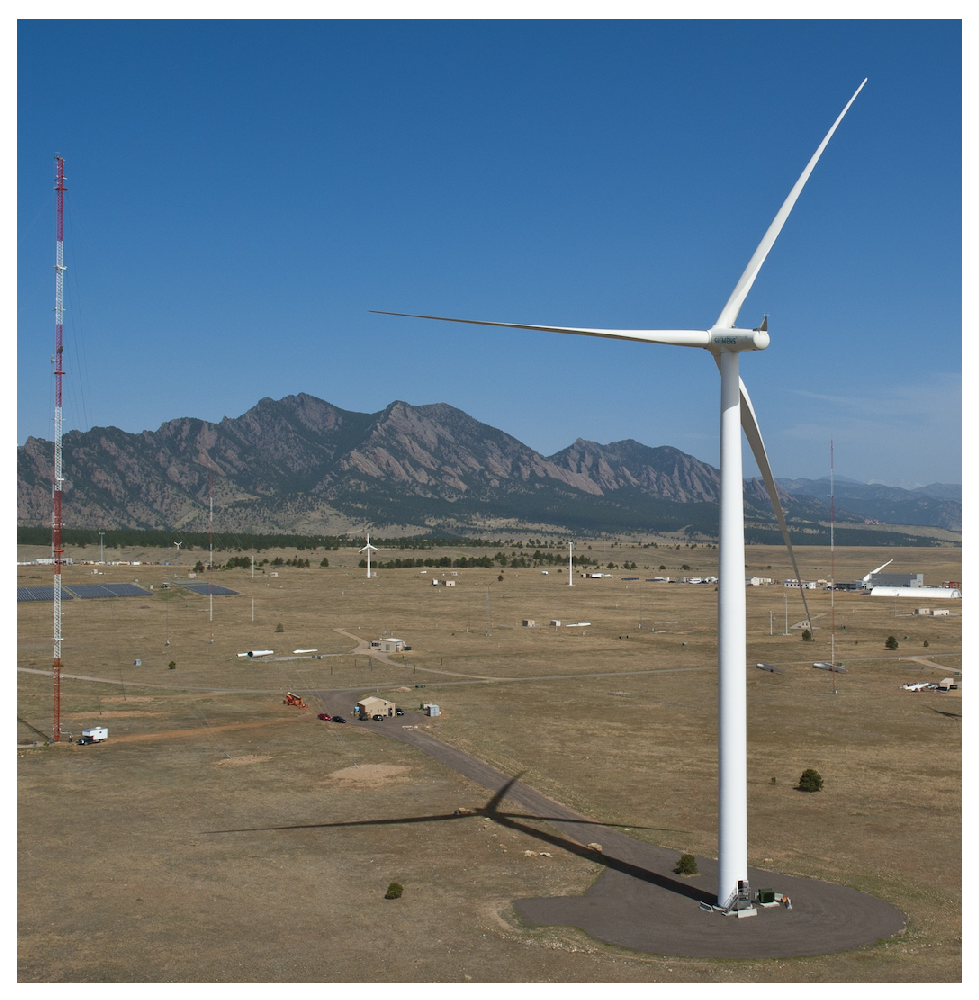
\includegraphics[height=2.5in]{files/20018}}
\hfill
\caption{NREL images}\label{fig:NRELimages}
\end{figure}
\end{verbatim}
 
\begin{figure*}[htp]
\centering
\hfill
\subfigure[Wind turbines at the Forward Wind Energy Center in Fond du Lac and Dodge Counties, Wisconsin. (Photo by Ruth Baranowski / NREL)\label{fig:21206}]{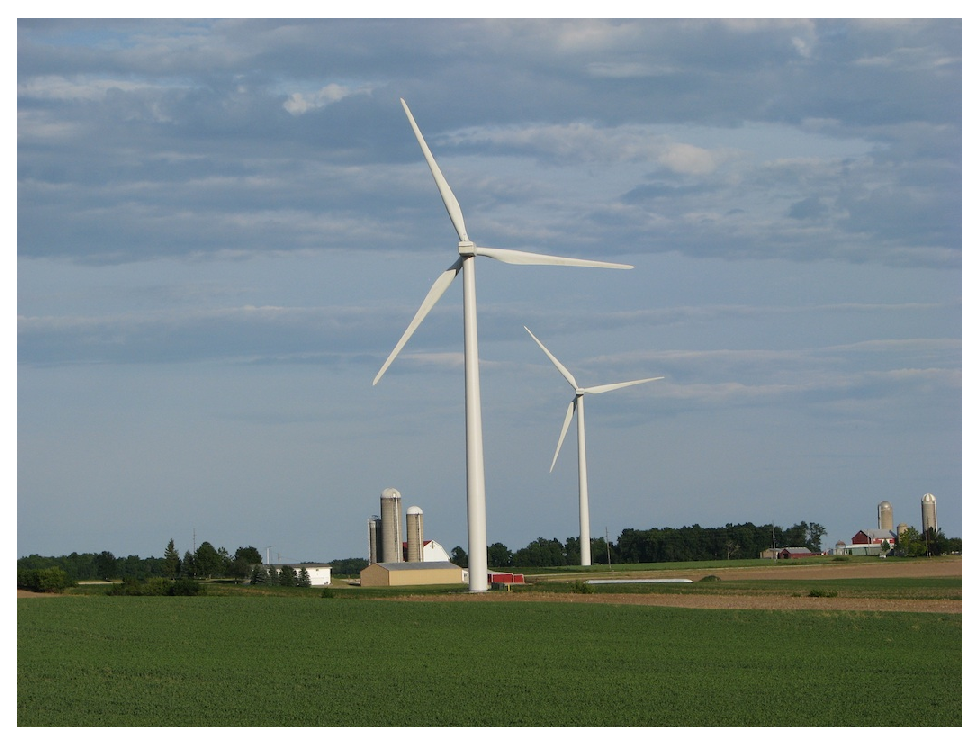
\includegraphics[height=2.5in]{files/21206.eps}}
~ %add desired spacing between images, e. g. ~, \quad, \qquad etc. (or a blank line to force the subfigure onto a new line)
\hfill
\subfigure[Aerial view of the National Wind Technology Center. (Photo by Dennis Schroeder / NREL)\label{fig:20018}]{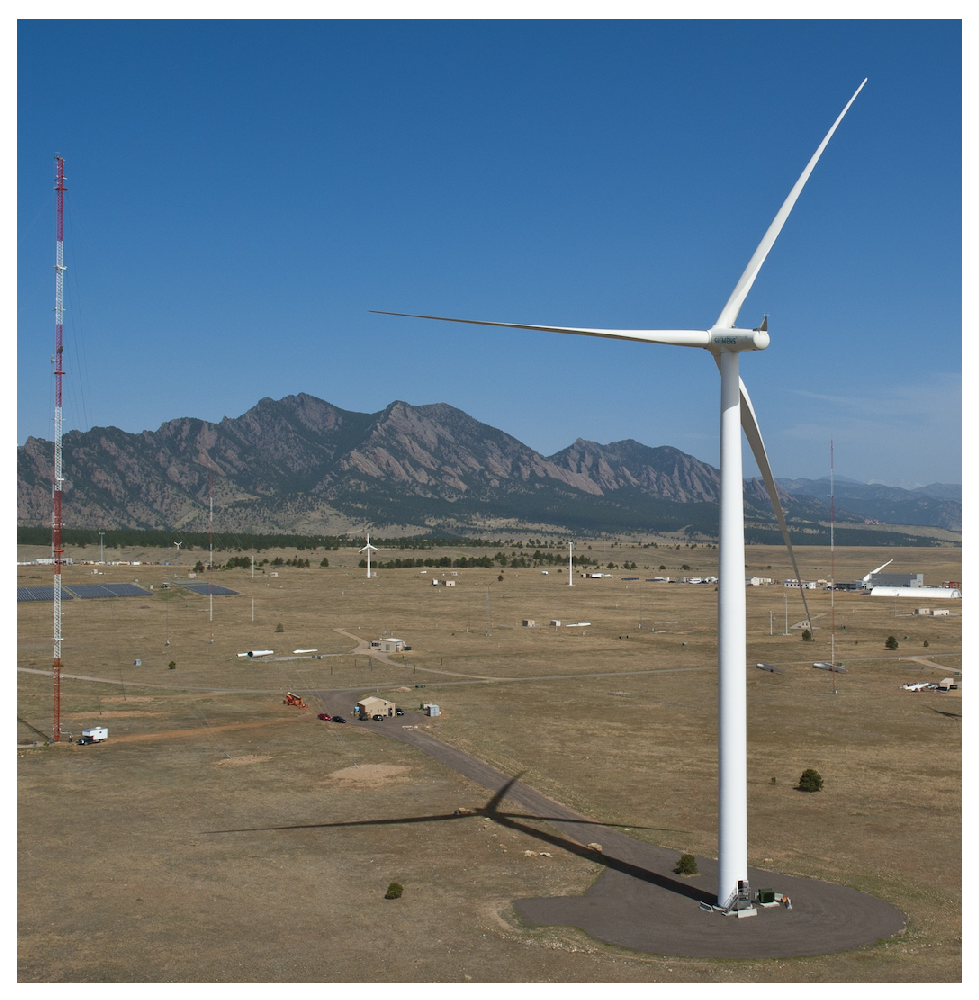
\includegraphics[height=2.5in]{files/20018.eps}}
\hfill
\caption{NREL images}\label{fig:NRELimages}
\end{figure*}

If a subfigure is split over two lines using \verb+\\+, make sure those symbols are on their own line.

\section{Lists}

To make lists with automatic numbering, use the \texttt{enumerate} environment:

\begin{enumerate}
\item Like this,
\item and like this.
\end{enumerate}
\dots or bullet points \dots
\begin{itemize}
\item Like this,
\item and like this.
\end{itemize}

\section{Computer code}
The \texttt{lstlisting} package has been loaded.

\section{Creating a file structure}
\label{sec:FileStructure}
Use the \texttt{input} command to import other files into your main file. For example, each of the chapters in this report could be in separate files, called \emph{NRELRequirements} (Chapter 1), \emph{LatexAtNREL} (Chapter 2), and so-on. 

\begin{verbatim}
...
% content
\input{NRELRequirements}
\input{LatexAtNREL}
\chapter{Some LaTeX examples}
This chapter includes examples of how to do common tasks using LaTeX{}. Although most users will be familiar with these commands and environments, these serve as a) a test of the class file and conversion process, and b) examples that are known to work with the class and conversion process. So, when all else fails, users can copy these examples and tailor them to their particular case.

\section{Headings}
LaTeX{} allows a very simple definition of the document's structure. This document has the following structure:
\begin{itemize}
\item Chapter 1: what is LaTeX?
\begin{itemize}
\item Section 1: Headings
\item Section 2: Floats
\item Section 3: Mathematics
\item Section 4: Lists
\end{itemize}
\item etc. \ldots
\end{itemize}

\subsection{Chapter}
To define a new chapter, simply write \verb+\chapter{What is LaTeX?}+.

To use chapters, pass the \texttt{memoir}, \texttt{book}, or \texttt{report} option to \emph{nrel.cls} (see Section \ref{sec:nrel.cls.options}).

\subsection{Sections}
If Chapters are the highest level headings in a document, sections come next, followed by subsections. Although there don't have to be chapters in a document, a LaTeX document does need to have Sections.

So: 

\begin{verbatim}
\section{Headings}
LaTeX{} allows a very simple definition of the document's structure. 
This document has the following structure:
...
\subsection{Chapter}

\end{verbatim}

\section{Body text}
Body text does not need to be specially identified in LaTeX{}. Non-printing comments are identified in the source document(s) using the \% symbol.

\section{Mathematics}

LaTeX is great at typesetting mathematics. The following example is taken from the \href{www.writelatex.com}{www.writelatex.com} website:

\begin{quote}
Making inline equations is easy. Let $X_1, X_2, \ldots, X_n$ be a sequence of independent and identically distributed random variables with $\textrm{E}[X_i] = \mu$ and $\textrm{Var}[X_i] = \sigma^2 < \infty$, and let
$$S_n = \frac{X_1 + X_2 + \cdots + X_n}{n}
 = \frac{1}{n}\sum_{i}^{n} X_i$$
denote their mean. Then as $n$ approaches infinity, the random variables $\sqrt{n}(S_n - \mu)$ converge in distribution to a normal $\mathcal{N}(0, \sigma^2)$.
\end{quote}

Alternatively, if numbered equations are required, use the \texttt{equation} environment. For example:

\begin{verbatim}
\begin{equation}
y = mx +c \textrm{.}
\label{eqn:line}
\end{equation}
\end{verbatim}

would give:

\begin{equation}
y = mx+c \textrm{.}
\label{eqn:line}
\end{equation}

\section{Cross references}
Use labels and references to refer back and forth to figures, equations, tables and sections. For example, \verb+Eqn. \ref{eqn:line}+ gives a reference to Eqn. \ref{eqn:line}.

\section{Floats}
Floats are images, tables or other pieces of the document that are free to move to the best place in the document for them. Literally, they `float'. The two most common floats are the tabular environment (for tables) and the figure environment for figures.

\subsection{Tables}
Use the \texttt{tabular} environment to produce basic tables. Table~\ref{tab:widgets} is produced using this code: 

\begin{verbatim}
\begin{table}[!h]
\centering
\caption{An example table.}\label{tab:widgets}
\begin{tabular}{lr}
Item & Quantity \\\hline
Widgets & 42 \\
Gadgets & 13
\end{tabular}
\end{table}
\end{verbatim}

\begin{table}[!h]
\centering
\caption{An example table.}\label{tab:widgets}
\begin{tabular}{lr}
Item & Quantity \\\hline
Widgets & 42 \\
Gadgets & 13
\end{tabular}
\end{table}

Resist the temptation to stop table rows early. If all of the delimiters  (\&) are included in each row, the table will be complete and will better translate to RTF later.

\subsection{Figures}
To include a figure in a document, use the \texttt{figure} environment and the \texttt{includegraphics} command.

\begin{verbatim}
\begin{figure}
\includegraphics[width=\textwidth]{figure's-file-name}
\caption{Caption goes here.}\label{fig:figuresLabel}
\end{figure}
\end{verbatim}

\subsection{Subfigures}
Subfigures are implemented using the \texttt{subfig} package. Although this package is deprecated (apparently \texttt{subcaption} is now the preferred package), it plays fairly nicely with \texttt{latex2rtf} so will be used for the foreseeable future. 

The \texttt{label}s in the example below allow us to make references using the \texttt{ref} command, both to the overall figure (Figure \ref{fig:NRELimages}) and the subfigures (Figures \ref{fig:21206} and \ref{fig:20018}) directly. Unfortunately, \texttt{latex2rtf} does not allow multiple \texttt{label}s in a Figure environment, and so only the first label will be kept: therefore, it's best to just use a single label in any one \texttt{figure} environment.

\begin{verbatim}
\begin{figure}
\centering
\hfill
\subfigure[Wind turbines at the Forward Wind Energy Center in Fond du Lac 
 and Dodge Counties, Wisconsin. (Photo by Ruth Baranowski / NREL)
 \label{fig:21206}]{\includegraphics[height=2.5in]{files/21206}}
\hfill 
\subfigure[Aerial view of the National Wind Technology Center. 
 (Photo by Dennis Schroeder / NREL)\label{fig:20018}]
 {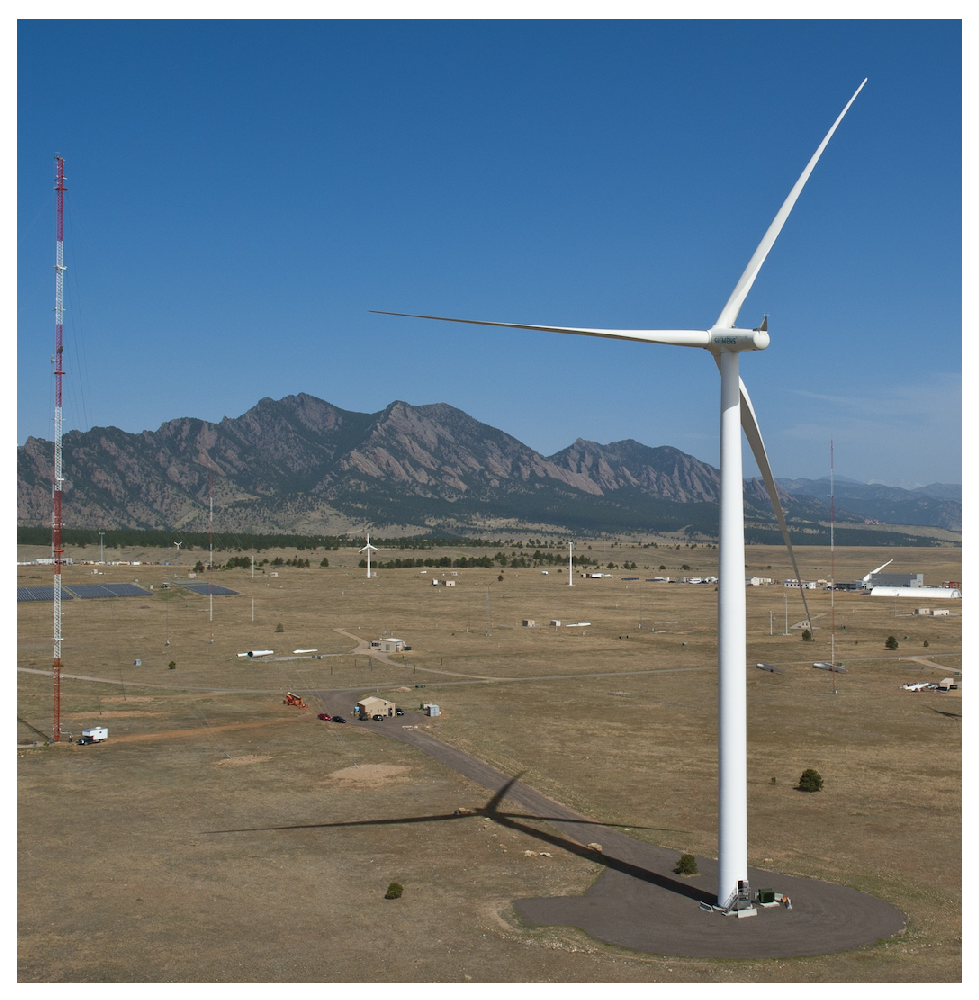
\includegraphics[height=2.5in]{files/20018}}
\hfill
\caption{NREL images}\label{fig:NRELimages}
\end{figure}
\end{verbatim}
 
\begin{figure*}[htp]
\centering
\hfill
\subfigure[Wind turbines at the Forward Wind Energy Center in Fond du Lac and Dodge Counties, Wisconsin. (Photo by Ruth Baranowski / NREL)\label{fig:21206}]{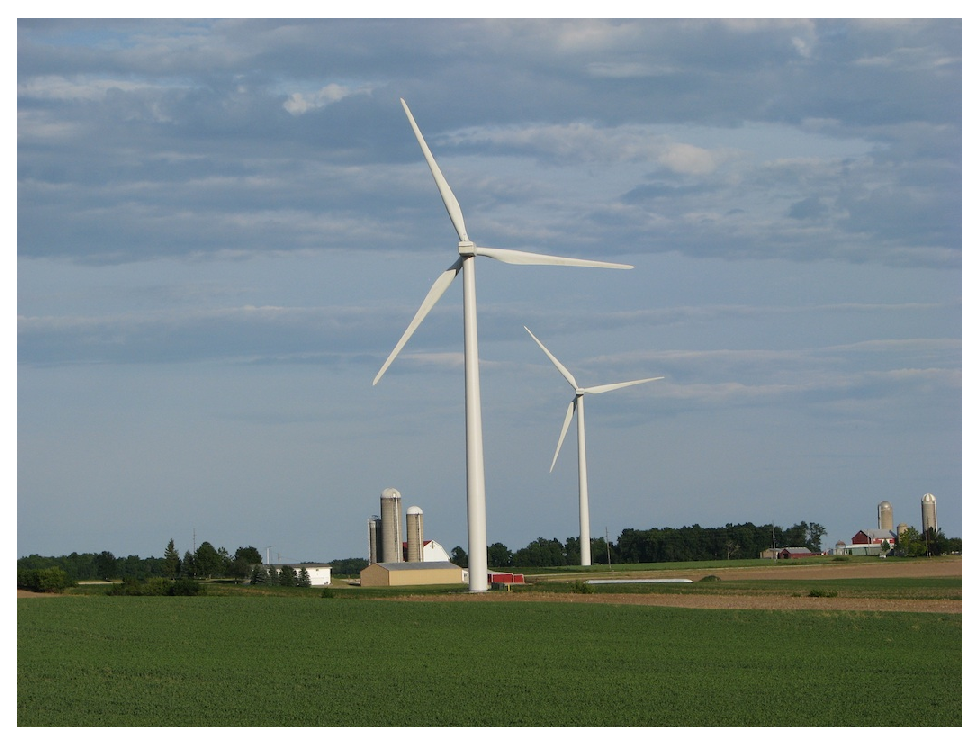
\includegraphics[height=2.5in]{files/21206.eps}}
~ %add desired spacing between images, e. g. ~, \quad, \qquad etc. (or a blank line to force the subfigure onto a new line)
\hfill
\subfigure[Aerial view of the National Wind Technology Center. (Photo by Dennis Schroeder / NREL)\label{fig:20018}]{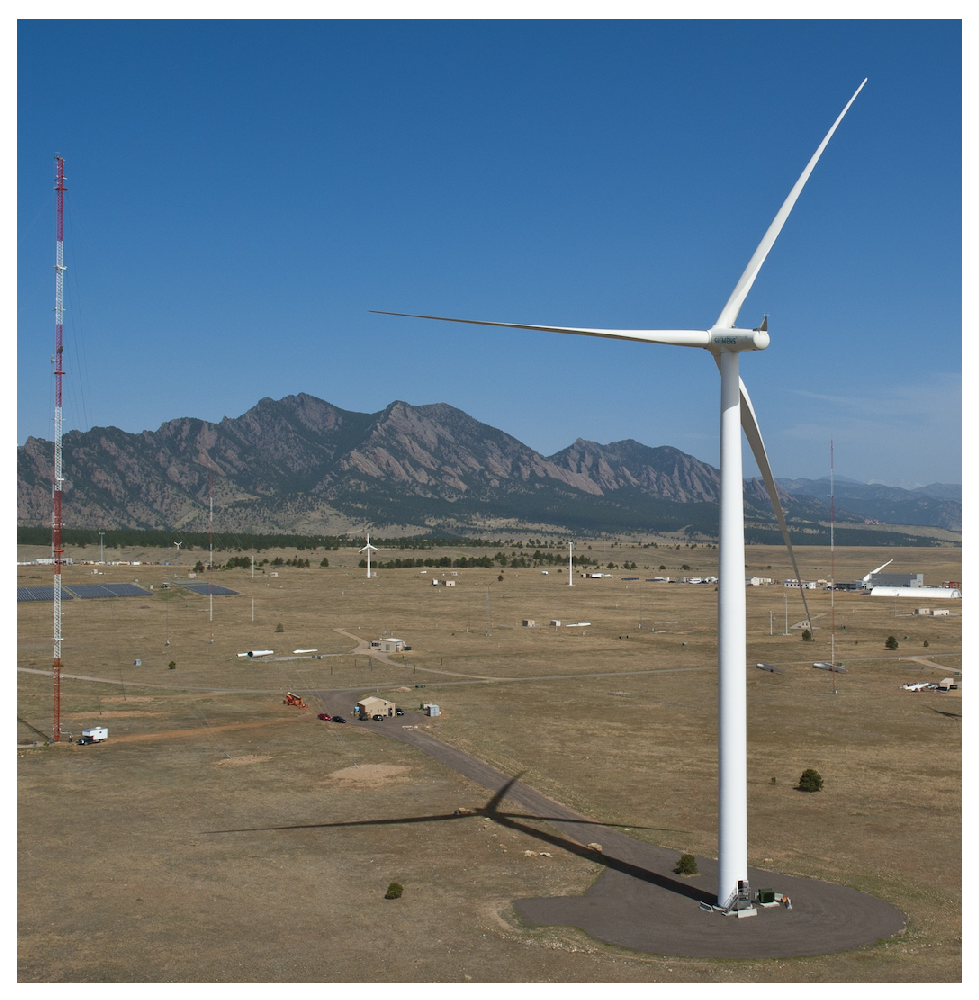
\includegraphics[height=2.5in]{files/20018.eps}}
\hfill
\caption{NREL images}\label{fig:NRELimages}
\end{figure*}

If a subfigure is split over two lines using \verb+\\+, make sure those symbols are on their own line.

\section{Lists}

To make lists with automatic numbering, use the \texttt{enumerate} environment:

\begin{enumerate}
\item Like this,
\item and like this.
\end{enumerate}
\dots or bullet points \dots
\begin{itemize}
\item Like this,
\item and like this.
\end{itemize}

\section{Computer code}
The \texttt{lstlisting} package has been loaded.

\section{Creating a file structure}
\label{sec:FileStructure}
Use the \texttt{input} command to import other files into your main file. For example, each of the chapters in this report could be in separate files, called \emph{NRELRequirements} (Chapter 1), \emph{LatexAtNREL} (Chapter 2), and so-on. 

\begin{verbatim}
...
% content
\input{NRELRequirements}
\input{LatexAtNREL}
\chapter{Some LaTeX examples}
This chapter includes examples of how to do common tasks using LaTeX{}. Although most users will be familiar with these commands and environments, these serve as a) a test of the class file and conversion process, and b) examples that are known to work with the class and conversion process. So, when all else fails, users can copy these examples and tailor them to their particular case.

\section{Headings}
LaTeX{} allows a very simple definition of the document's structure. This document has the following structure:
\begin{itemize}
\item Chapter 1: what is LaTeX?
\begin{itemize}
\item Section 1: Headings
\item Section 2: Floats
\item Section 3: Mathematics
\item Section 4: Lists
\end{itemize}
\item etc. \ldots
\end{itemize}

\subsection{Chapter}
To define a new chapter, simply write \verb+\chapter{What is LaTeX?}+.

To use chapters, pass the \texttt{memoir}, \texttt{book}, or \texttt{report} option to \emph{nrel.cls} (see Section \ref{sec:nrel.cls.options}).

\subsection{Sections}
If Chapters are the highest level headings in a document, sections come next, followed by subsections. Although there don't have to be chapters in a document, a LaTeX document does need to have Sections.

So: 

\begin{verbatim}
\section{Headings}
LaTeX{} allows a very simple definition of the document's structure. 
This document has the following structure:
...
\subsection{Chapter}

\end{verbatim}

\section{Body text}
Body text does not need to be specially identified in LaTeX{}. Non-printing comments are identified in the source document(s) using the \% symbol.

\section{Mathematics}

LaTeX is great at typesetting mathematics. The following example is taken from the \href{www.writelatex.com}{www.writelatex.com} website:

\begin{quote}
Making inline equations is easy. Let $X_1, X_2, \ldots, X_n$ be a sequence of independent and identically distributed random variables with $\textrm{E}[X_i] = \mu$ and $\textrm{Var}[X_i] = \sigma^2 < \infty$, and let
$$S_n = \frac{X_1 + X_2 + \cdots + X_n}{n}
 = \frac{1}{n}\sum_{i}^{n} X_i$$
denote their mean. Then as $n$ approaches infinity, the random variables $\sqrt{n}(S_n - \mu)$ converge in distribution to a normal $\mathcal{N}(0, \sigma^2)$.
\end{quote}

Alternatively, if numbered equations are required, use the \texttt{equation} environment. For example:

\begin{verbatim}
\begin{equation}
y = mx +c \textrm{.}
\label{eqn:line}
\end{equation}
\end{verbatim}

would give:

\begin{equation}
y = mx+c \textrm{.}
\label{eqn:line}
\end{equation}

\section{Cross references}
Use labels and references to refer back and forth to figures, equations, tables and sections. For example, \verb+Eqn. \ref{eqn:line}+ gives a reference to Eqn. \ref{eqn:line}.

\section{Floats}
Floats are images, tables or other pieces of the document that are free to move to the best place in the document for them. Literally, they `float'. The two most common floats are the tabular environment (for tables) and the figure environment for figures.

\subsection{Tables}
Use the \texttt{tabular} environment to produce basic tables. Table~\ref{tab:widgets} is produced using this code: 

\begin{verbatim}
\begin{table}[!h]
\centering
\caption{An example table.}\label{tab:widgets}
\begin{tabular}{lr}
Item & Quantity \\\hline
Widgets & 42 \\
Gadgets & 13
\end{tabular}
\end{table}
\end{verbatim}

\begin{table}[!h]
\centering
\caption{An example table.}\label{tab:widgets}
\begin{tabular}{lr}
Item & Quantity \\\hline
Widgets & 42 \\
Gadgets & 13
\end{tabular}
\end{table}

Resist the temptation to stop table rows early. If all of the delimiters  (\&) are included in each row, the table will be complete and will better translate to RTF later.

\subsection{Figures}
To include a figure in a document, use the \texttt{figure} environment and the \texttt{includegraphics} command.

\begin{verbatim}
\begin{figure}
\includegraphics[width=\textwidth]{figure's-file-name}
\caption{Caption goes here.}\label{fig:figuresLabel}
\end{figure}
\end{verbatim}

\subsection{Subfigures}
Subfigures are implemented using the \texttt{subfig} package. Although this package is deprecated (apparently \texttt{subcaption} is now the preferred package), it plays fairly nicely with \texttt{latex2rtf} so will be used for the foreseeable future. 

The \texttt{label}s in the example below allow us to make references using the \texttt{ref} command, both to the overall figure (Figure \ref{fig:NRELimages}) and the subfigures (Figures \ref{fig:21206} and \ref{fig:20018}) directly. Unfortunately, \texttt{latex2rtf} does not allow multiple \texttt{label}s in a Figure environment, and so only the first label will be kept: therefore, it's best to just use a single label in any one \texttt{figure} environment.

\begin{verbatim}
\begin{figure}
\centering
\hfill
\subfigure[Wind turbines at the Forward Wind Energy Center in Fond du Lac 
 and Dodge Counties, Wisconsin. (Photo by Ruth Baranowski / NREL)
 \label{fig:21206}]{\includegraphics[height=2.5in]{files/21206}}
\hfill 
\subfigure[Aerial view of the National Wind Technology Center. 
 (Photo by Dennis Schroeder / NREL)\label{fig:20018}]
 {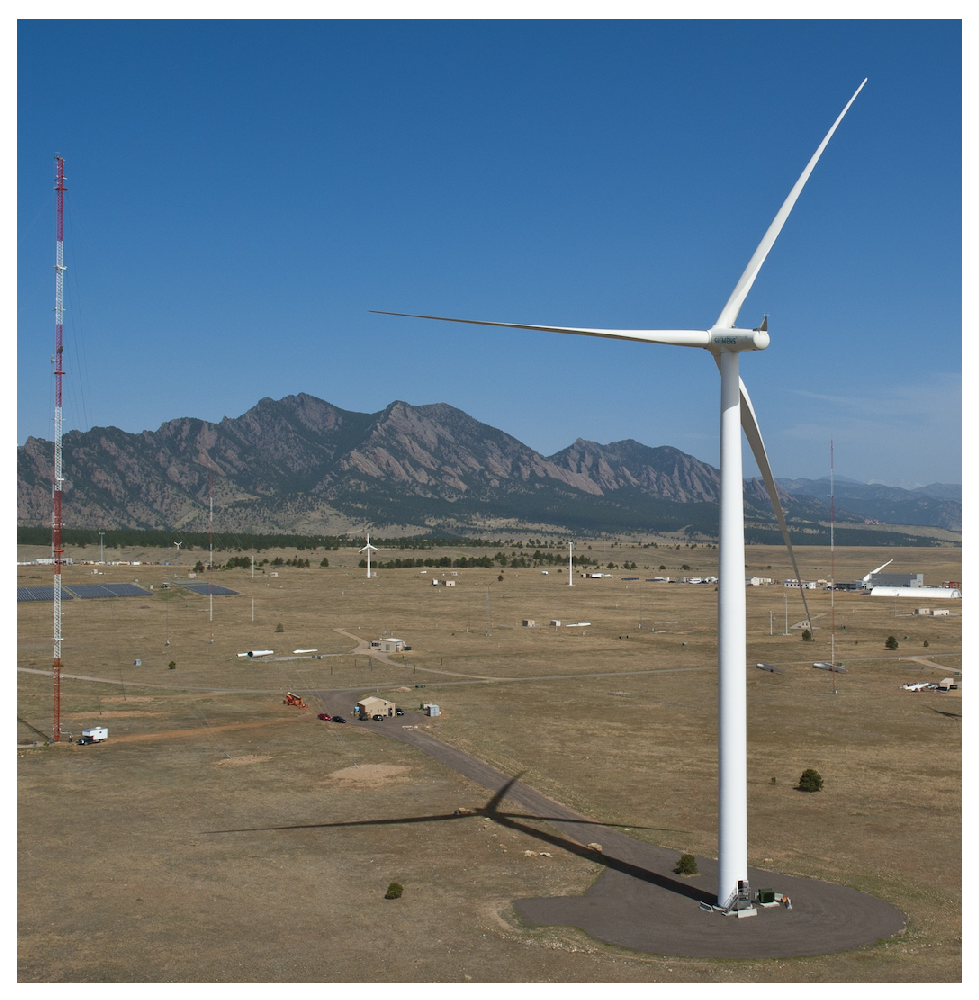
\includegraphics[height=2.5in]{files/20018}}
\hfill
\caption{NREL images}\label{fig:NRELimages}
\end{figure}
\end{verbatim}
 
\begin{figure*}[htp]
\centering
\hfill
\subfigure[Wind turbines at the Forward Wind Energy Center in Fond du Lac and Dodge Counties, Wisconsin. (Photo by Ruth Baranowski / NREL)\label{fig:21206}]{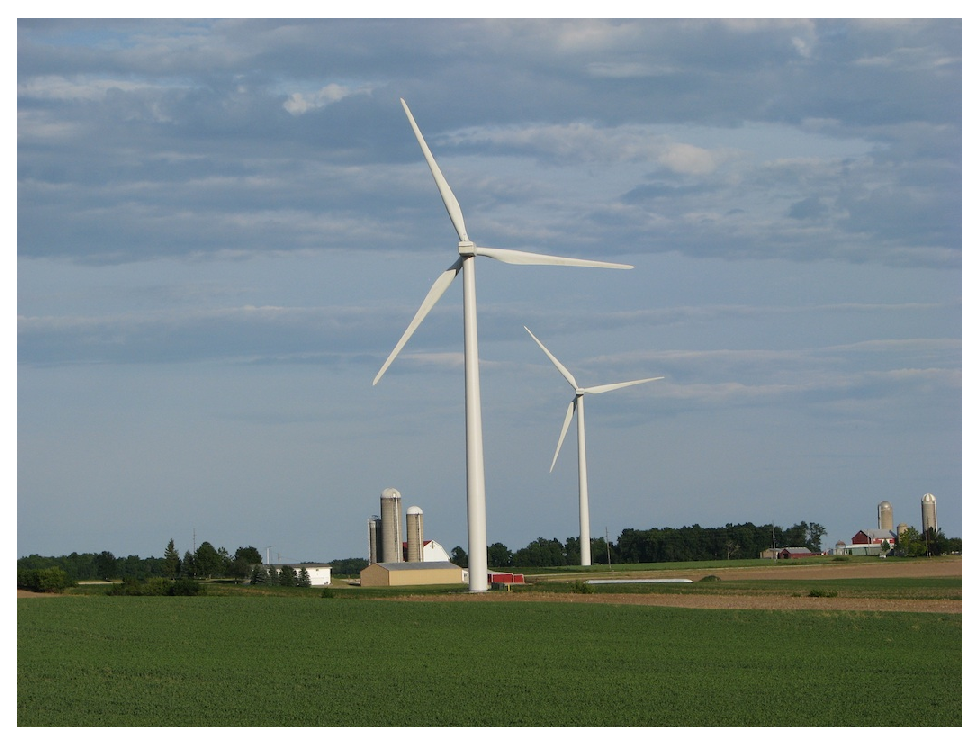
\includegraphics[height=2.5in]{files/21206.eps}}
~ %add desired spacing between images, e. g. ~, \quad, \qquad etc. (or a blank line to force the subfigure onto a new line)
\hfill
\subfigure[Aerial view of the National Wind Technology Center. (Photo by Dennis Schroeder / NREL)\label{fig:20018}]{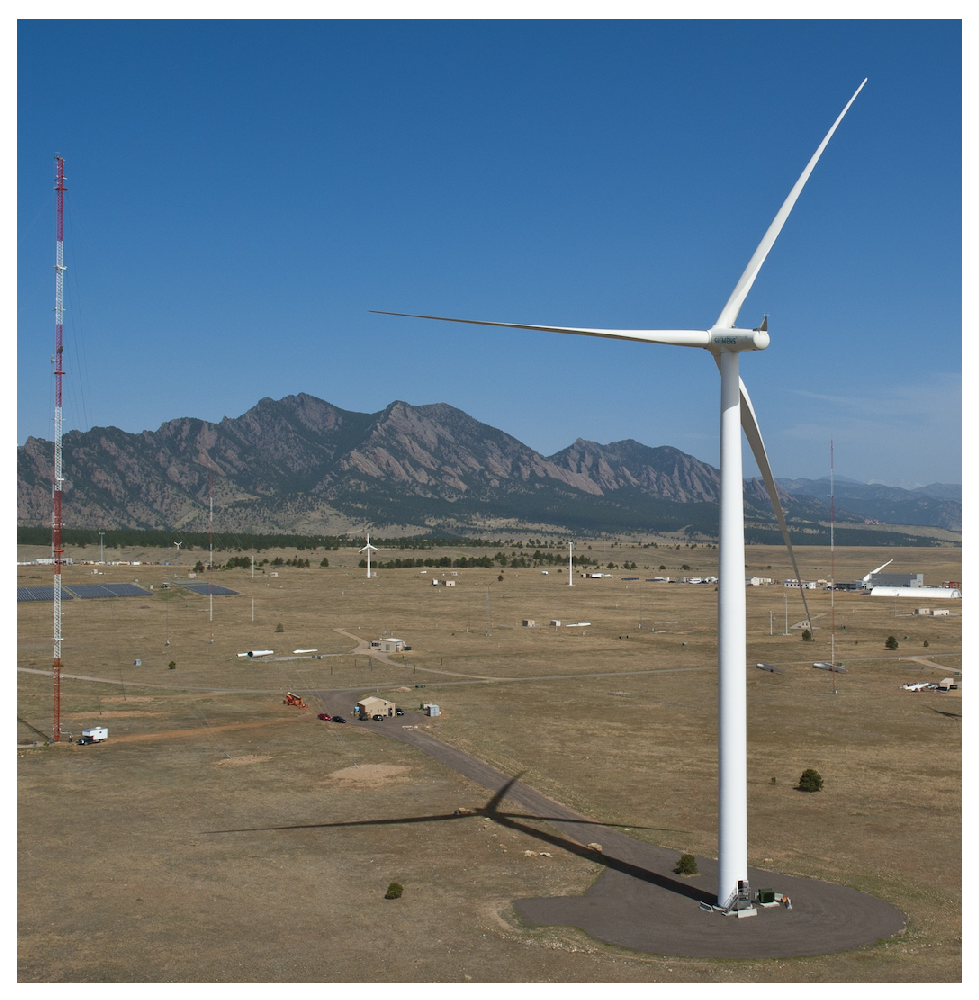
\includegraphics[height=2.5in]{files/20018.eps}}
\hfill
\caption{NREL images}\label{fig:NRELimages}
\end{figure*}

If a subfigure is split over two lines using \verb+\\+, make sure those symbols are on their own line.

\section{Lists}

To make lists with automatic numbering, use the \texttt{enumerate} environment:

\begin{enumerate}
\item Like this,
\item and like this.
\end{enumerate}
\dots or bullet points \dots
\begin{itemize}
\item Like this,
\item and like this.
\end{itemize}

\section{Computer code}
The \texttt{lstlisting} package has been loaded.

\section{Creating a file structure}
\label{sec:FileStructure}
Use the \texttt{input} command to import other files into your main file. For example, each of the chapters in this report could be in separate files, called \emph{NRELRequirements} (Chapter 1), \emph{LatexAtNREL} (Chapter 2), and so-on. 

\begin{verbatim}
...
% content
\input{NRELRequirements}
\input{LatexAtNREL}
\input{LatexExamples}
\input{ConvertingToDoc}
...
\end{verbatim}

\input{ConvertingToDoc}
...
\end{verbatim}

\input{ConvertingToDoc}
...
\end{verbatim}

%% CHAPTER:MAKING DOC FILES
%\chapter{Preparing a .DOC or .DOCX file from LaTeX}\label{sec:latextodoc}
LaTeX users may find that they are required to convert their files into other formats for review or  editing. This section describes how LaTeX files can be converted into files that can be used with Microsoft Word.

\section{The conversion process} 
The NREL style has been designed to be converted into \emph{.doc} or \emph{.docx}. This can be achieved via one of two routes:
\begin{enumerate}
\item converting the latex file to rich text format (\emph{.rtf}) using \texttt{latex2rtf}, then importing the file into a word processor, or
\item converting the latex file to doc using pandoc.
\end{enumerate}

The performance of \texttt{Latex2rtf} and \texttt{pandoc} are compared in Table \ref{tab:conversioncomparison}.

\begin{table}[!h]
\centering
\caption{A comparison of latex2rtf and pandoc for document conversion.}\label{tab:conversioncomparison}
\begin{tabular}{lcc}
consideration & latex2rtf & pandoc \\\hline
requires changes to latex preamble & yes & no\\
output format & .rtf & .docx \\
supports cross references & yes & no\\
supports subfigures & partially & no\\
\end{tabular}
\end{table}

At this time, \texttt{latex2rtf} is the recommended tool for converting LaTeX files that have been made with the NREL class file, into word processor-readable files.

\section{Using latex2rtf to convert files}
The \texttt{latex2rtf} program reads LaTeX files and converts common LaTeX commands into their RTF equivalent. It is effectively another LaTeX interpreter that knows a limited subset of LaTeX. See the documentation at \href{http://sourceforge.net/projects/latex2rtf/}{http://sourceforge.net/projects/latex2rtf/} for details.

\subsection{Using latex2rtf}
To convert a document from LaTeX to RTF, follow these steps:
\begin{enumerate}
\item Install \texttt{latex2rtf}
\item Compile the document in LaTeX using the NREL class with the \texttt{book,report}, or \texttt{article} option, remembering to update the bibliography and cross references. The sequence of commands is:
\item Convert the document to RTF format using \texttt{latex2rtf}. The example .rtf file included with this document is created as follows:
\begin{verbatim}
latex2rtf -o latex2rtf_demo.rtf -f3 intro_to_NREL_latex
\end{verbatim}
\item Open the RTF file in Microsoft Word.
\item If the document contains tables of contents, tables of figures, tables of tables, or cross-references, select that text and update the fields.
\item Save the RTF file as a word-format document.
\end{enumerate}

\subsection{Using latex2rtf and LaTeX together}
Because \texttt{latex2rtf} only knows a subset of LaTeX, it is important to account for this when preparing a LaTeX document. The biggest problem is the lack of many packages, which is why authors are encouraged to use the NREL class file, which is known to work well with \texttt{latex2rtf}. Sometimes, though, it is important to be able to remove formatting for compatibility with \texttt{latex2rtf}, and so the preamble to this document includes a check to see if \texttt{latex2rtf} is being used:

\begin{verbatim}
\newif\iflatextortf
\iflatextortf
	\documentclass[12pt,letterpaper]{report}
	% File NRELLatex2rtf.tex

% set margins
\usepackage[margin=1 in,letterpaper]{geometry}

% use citations
\usepackage[sort]{natbib}

% change the heading of the bibliography
\renewcommand{\bibsection}{\section{References}}

% redefine \pdftooltip so that it behaves differently with and without latextortf
\newcommand{\pdftooltip}[3][]{#2}

%redefine the checkmark
\newcommand{\checkmark}{y\relax}

% redefine booktabs commands
\newcommand{\toprule}{\hline}
\newcommand{\midrule}{\hline}
\newcommand{\bottomrule}{\hline}

% redefine \href
\newcommand{\href}[2]{#1~ (\url{#2})}

% redefine \subfloat to match the \subfigure environment
\usepackage{subfigure}
\makeatletter
\newcommand{\subfloat}[2][]{\subfigure{\textit{Subcaption: \protect{#1}}}{#2}}
%\newcommand{\subfloat}[3][]{\subfigure{#1}{#2}{#3}}
% note that we can only have one '\label' in a figure environment
\makeatother

\newcommand{\subref}[1][]{\ref{#1}}

% redefine \todo so that it gives something useful
\newcommand{\todo}[2][]{\textbf{To Do:}~#2}

% deal with index entries:
\newcommand{\index}[1]{}
\else
	\documentclass[report]{nrel} 
\fi
\end{verbatim}

If \texttt{latex2rtf} is used, the boolean, \texttt{\textbackslash iflatextortf} will be TRUE and the commands will be interpreted as follows.
\begin{enumerate}
\item Set the document class to a generic LaTeX{} \emph{article}, \emph{report}, or \emph{book}. 
\item The file \emph{NRELLatex2rtf.tex} will be called, which maps most of the commands that are enabled in \emph{nrel.cls} to simpler versions that can be processed using \texttt{latex2rtf} (see Table \ref{Tab:Packages}).
\end{enumerate}

Authors that use packages other than those listed in Table \ref{Tab:Packages} may need to adjust the content of \emph{NRELLatex2rtf.tex} according to their needs. 

\subsection{Indexes}
Index entries will not be correctly converted to an \emph{.rtf} file. \emph{NRELLatex2rtf.tex} redefines the \verb+index+ command to do nothing when creating an \emph{.rtf} file. 

\subsection{What to do when the conversion to rich text format fails}
It is more than likely that the conversion to an \emph{.rtf} file will fail at some point. There are a few ways to deal with this:

\begin{description}
\item[Convert early and often.] Check that the document converts using \texttt{latex2rtf} every time a new environment is added.
\item[Try section-by-section.] Comment out the majority of the document and try to compile bit-by-bit. This will let you localize the error.
\item[Check new packages.] Please avoid using new packages. If a package has to be used, try the conversion immediately. If \texttt{latex2rtf} doesn't support the package, edit the file \emph{NRELLatex2rtf.tex} to redefine those commands to something that will convert appropriately. Put \emph{NRELLatex2rtf.tex} in the same directory as the LaTeX file to be converted.
\item[Avoid custom commands.] \texttt{latex2rtf} sometimes chokes on custom commands. A list of all recognized commands is available in the manual at \href{http://latex2rtf.sourceforge.net/latex2rtf.pdf}{http://latex2rtf.sourceforge.net/latex2rtf.pdf}. If custom commands are used, they may need to be redefined to work with the commands that \texttt{latex2rtf} does recognize. This can also be done in \emph{NRELLatex2rtf.tex}. You can check macros using the flag \verb+-d2+ when running \texttt{latex2rtf}.
\item[Use copy-paste.] Compile the whole document as a PDF, and save it somewhere. Then recompile using the reduced document that works with \texttt{latex2rtf}. Edit this in word and copy in the bits that killed the conversion.
\item[Talk to a communications rep.] If a document cannot be produced any other way than LaTeX with lots of packages, and \texttt{latex2rtf} just refuses to process it into a rich text file, discuss the process for having the PDF processed.
\end{description}

\section{Using pandoc}
Pandoc is a tool for converting documents between different formats. Pandoc is available at \href{http://johnmacfarlane.net/pandoc/}{http://johnmacfarlane.net/pandoc/}. Like \texttt{latex2rtf}, pandoc only supports a subset of latex commands and is not guaranteed to work for all applications.

Pandoc has several advantages over latex2rtf:
\begin{itemize}
\item Pandoc it supports conversion from latex to many other document formats (e.g. .html as well as .docx). However, there are other well-established tools to go directly from latex source code to other formats that may have better performance.
\item Pandoc does not require any changes to the latex source files.
\end{itemize}

To use pandoc, follow the installation instructions on the pandoc website, and then run pandoc from the command line. To convert this file, use the following command at the command line:

\begin{verbatim}
pandoc -o conversion_demo/pandoc_demo.docx intro_to_NREL_latex.tex --bibliography bibliography.bib --default-image-extension=.jpg
\end{verbatim}


%% CHAPTER: MAKING PDFS
%\chapter{Preparing a high-quality PDF from LaTeX}\label{sec:PDFprep}
If the author chooses to complete the publications process using LaTeX\, the author must incorporate feedback and edits in to the LaTeX source files and prepare the final PDF, following these guidelines.

\section{PDF tagging}\label{sec:PDFtagging}
PDF tagging is a process whereby the components of the PDF document (headings, figures, tables, text) are marked so that a document reader can understand the document. This is useful when text to speech converters are being used. The process of tagging is also known as structuring, so that a tagged document might also be referred to as a structured document.

LaTeX does not prepare a tagged PDF document. The current solution to this is to use the tagging capability built in to Adobe's Acrobat Pro.

To prepare a tagged document, follow these steps:
\begin{enumerate}
\item Add tags. Go to the `Advanced' menu. Select `Accessibility', then `Add tags to document'.
\item Add alternative text for figures. Context-click the Figure, select `Properties', and fill in `Alternate Text'. Alternatively, try the process outlined below.
\item Specify the document language. Go to the `File' menu. Select `Document Properties', then the `Advanced' tab, `Language' field. In some versions of Acrobat, the sequence is `File', `Properties', `Reading Options', `Language'.
\item Define tab order.
\begin{enumerate}
\item Go to the `View' menu. Select `Navigation tabs', then `Pages'.
\item Click on any page, then type Ctrl-A (or Command-A on a Mac) to select all the pages.
\item Go to the `Options' menu in the top right of the dialog box, and select `Page Properties'
\item In the `Tab Order' tab, select `Use document structure'.
\end{enumerate}
\item Make sure tables have headings. 
\begin{enumerate}
\item Go to the `View' menu. Select `Navigation tabs', then `Tags'.
\item Select the `Tags' tab. This panel shows the document structure as a tree.
\item Navigate to the table cells that should be headers.
\item Check they have the type <TH>. If not, then right click on the header cell, select `properties', select the `Tag' tab, and change the value for `Type' to <TH>.
\end{enumerate}
\item Make sure all Chapters (or sections, if there are no chapters in the document) are correctly tagged.
\end{enumerate}

\section{Alt-text on images and equations}
`Alt text' is a textual description of an equation, link or figure. The following short equation should pop-up some text when a user passes a mouse over it. This should work in most PDF readers:
\begin{equation}
\pdftooltip{a^2+b^2=c^2}{An equation}
%a^2+b^2=c^2
\end{equation}

The alt text can be added after the PDF is compiled, or written in to the source document. The rest of this section describes how it can be added to the source and generated by LaTeX using the \href{pdfcomment}{http://www.ctan.org/pkg/pdfcomment} package. The general form of the command is:

\begin{verbatim}
\pdftooltip{<item>}{<pop-up text>}
\end{verbatim}

The previous equation was generated using this code:

\begin{verbatim}
\begin{equation}
\pdftooltip{a^2+b^2=c^2}{An equation}
\end{equation}
\end{verbatim}

The same approach can be used to create alt-text for images. For example, Figure \ref{fig:NRELimagesWithAltText} has been labeled. The code for this image is:

\begin{verbatim}
\begin{figure}[!h]
\centering
\hfill
\subfigure[Wind turbines at the Forward Wind Energy Center in Fond du Lac and Dodge Counties, Wisconsin. (Photo by Ruth Baranowski / NREL)] {\pdftooltip{\includegraphics[height=2.5in]{files/21206}}{This is an image}}
~ 
\hfill
\subfigure[Aerial view of the National Wind Technology Center.  (Photo by Dennis Schroeder / NREL)] {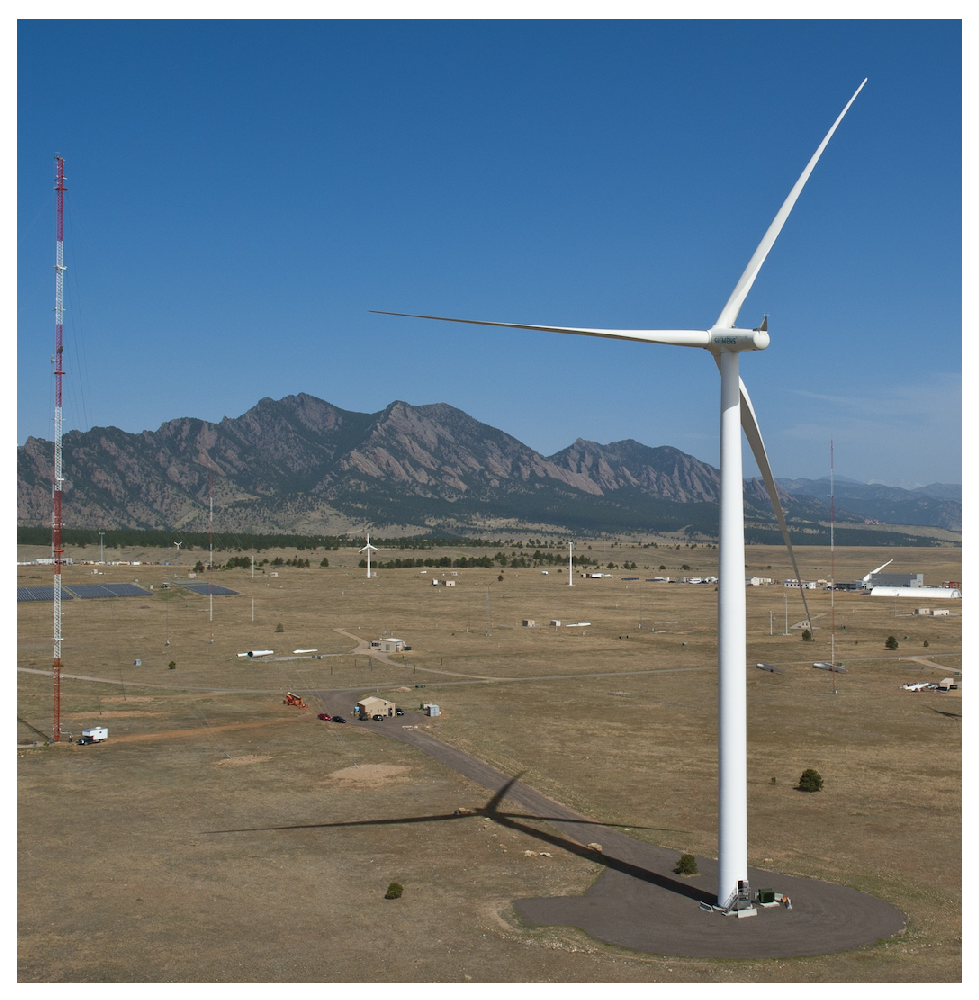
\includegraphics[height=2.5in]{files/20018}}
\hfill
\caption{NREL images}\label{fig:NRELimagesWithAltText}
\end{figure}
\end{verbatim}

\begin{figure}[!h]
\centering
\hfill
\subfigure[Wind turbines at the Forward Wind Energy Center in Fond du Lac and Dodge Counties, Wisconsin. (Photo by Ruth Baranowski / NREL)]{\pdftooltip{\includegraphics[height=2.5in]{files/21206}}{This is an image. It may be possible to propagate the caption into this text.}}
%{\includegraphics[height=2.5in]{21206}}
~ %add desired spacing between images, e. g. ~, \quad, \qquad etc. (or a blank line to force the subfigure onto a new line)
\hfill
\subfigure[Aerial view of the National Wind Technology Center. (Photo by Dennis Schroeder / NREL)]{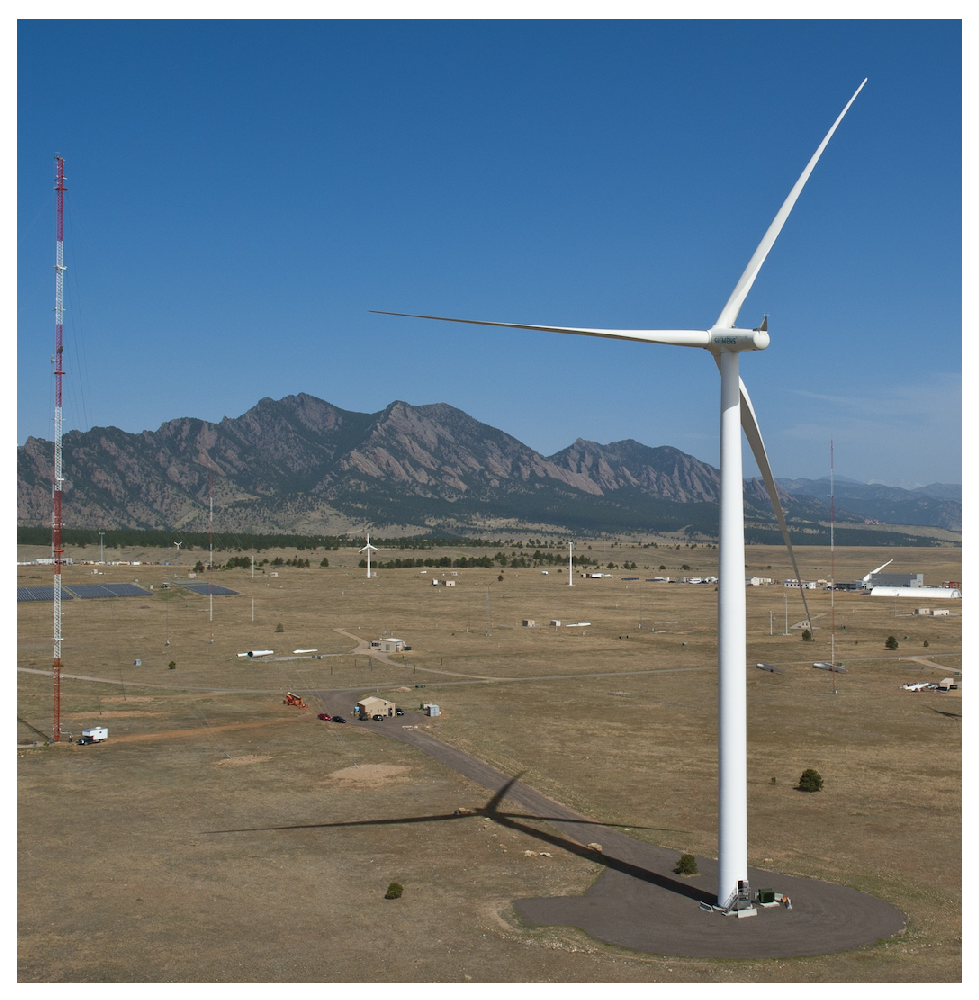
\includegraphics[height=2.5in]{files/20018}}
\hfill
\caption{NREL images}\label{fig:NRELimagesWithAltText}
\end{figure}

Alt-text is not processed by \texttt{latex2rtf}. So, if the author anticipates finishing the publication solely as a .DOC or .DOCX file, they do not need to use alt-text.

\section{Embedded fonts}
NREL requires that all fonts be embedded in the the final PDF. Check the PDF for embedded fonts using a PDF viewer. For example, in Adobe Acrobat Reader, look at the `fonts' tag of the document properties. If any fonts are not shown as being an \emph{embedded subset}, try the conversion again. 

Encapsulated postscript figures are particularly prone to having undefined fonts. Check by compiling the document in draft mode, and seeing if the fonts are still present in the output PDF. To fix this problem, consider changing the \emph{.eps} file to a \emph{.png}. To do this `on the fly', use this in the document's preamble:

\begin{verbatim}
\usepackage{epstopdf}
\epstopdfDeclareGraphicsRule
 {.eps}{png}{.png}{convert eps:\SourceFile.\SourceExt png:\OutputFile}
\AppendGraphicsExtensions{.png}
\end{verbatim}

% bibliography
\cleardoublepage
\bibliographystyle{nrel}
%\bibintoc
\label{sec:Bib}
\bibliography{files/bibliography}

\end{document}